\documentclass{letnab}
\pagestyle{fancy}
\usepackage{tabu}
\usepackage{units}
\usepackage{lscape}
\usepackage{ctable} % for \specialrule command
\usepackage{ulem}
\hyphenpenalty=1000
\usepackage{booktabs}
\rhead{Общая физика МФТИ}
\lhead{Экзамен: термодинамика} 

\renewcommand{\headrulewidth}{0.5pt}
\newcommand{\RomanNumeralCaps}[1]
{\MakeUppercase{\romannumeral #1}}

\newcommand{\chpr}[3]{\left(\dfrac{\partial #1}{\partial #2}\right)_#3}
\newcommand{\Chpr}[3]{\left(\frac{\partial #1}{\partial #2}\right)_#3}
\newcommand{\vtchpr}[4]{\dfrac{\partial}{\partial #1}\left(\dfrac{\partial #2}{\partial #3}\right)_#4}
\newcommand{\infint}{\int_{-\infty}^{+\infty}}

\usepackage{hyperref}
\usepackage{upgreek}
\usepackage{wrapfig}
\usepackage{lipsum}
\usepackage{cancel}

\hypersetup{pdfstartview=FitH,  linkcolor=linkcolor,urlcolor=urlcolor, 
	colorlinks=true}

% Цвета для гиперссылок
\usepackage{xcolor}


\definecolor{linkcolor}{HTML}{000000} % цвет ссылок
\definecolor{urlcolor}{HTML}{0000FF} % цвет гиперссылок


\setcounter{tocdepth}{1}

\begin{document}


	\begin{titlepage}
		

		
		
		\center % Center everything on the page
		
		
		
		%----------------------------------------------------------------------------------------
		%	HEADING SECTIONS
		%----------------------------------------------------------------------------------------
		
		\textsc{\LARGE Московский Физико-Технический Институт}\\[1,5cm] % Name of your university/college
		% Major heading such as course name
		\textsc{\Large Кафедра общей физики}\\[0.5cm]
		\textsc{\large Экзамен: термодинамика}\\[0.5cm] % Minor heading such as course title
		
		%----------------------------------------------------------------------------------------
		%	TITLE SECTION
		%----------------------------------------------------------------------------------------
		

		
		
		
		%----------------------------------------------------------------------------------------
		%	AUTHOR SECTION
		%----------------------------------------------------------------------------------------
		
			\begin{center} \large
				\emph{Автор:} \href{https://vk.com/domrachev_alexey}{Алексей \textsf{Домрачев}}\\
				Благодарю за неоценимую помощь: \href{https://vk.com/shevtsovalexey}{Алексея \textsf{Шевцова}}, \href{https://vk.com/uteshevia}{Ивана \textsf{Утешева}} и \href{https://vk.com/detinin_roman}{Романа \textsf{Детинина}}
			\end{center}

		
		
		\begin{bottompar}
			
\includegraphics[width = 80 mm]{logo.png}	\\[1,0cm]
			{\large \today}
		\end{bottompar}
		\vfill % Fill the rest of the page with whitespace
		
	\end{titlepage}



\tableofcontents
\newpage

 \section{\normalsize Термодинамическая система. Микроскопические и макроскопические параметры. Уравнение состояния (термическое и калорическое). Стационарные, равновесные и неравновесные состояния и процессы. }
\paragraph{Термодинамическая система.}\textbf{Cистема} --- совокупность рассматриваемых тел(\textit{частиц}), которые могут взаимодействовать между собой и с другими телами(\textit{внешняя среда}) посредством обмена веществом и энергией.\\
В термодинамике рассматриваются большие системы, называемые \textbf{термодинамическими системами}.
\paragraph{Микроскопическое состояние и макроскопическое состояние.}\textbf{Микроскопическое состояние} --- состояние системы, определяемое заданием координат и импульсов (\textit{микропараметры}) всех составляющих систему частиц.\\
\textbf{Макроскопическое состояние} --- состояние системы, характеризующееся небольшим числам макропараметров($P$, $V$, $T$, $\rho$, $\eta$ и т.д.). Макропараметры подразделяются на внутренние и внешние.
\paragraph{Уравнение состояния (термическое и калорическое).}\textbf{Уравнение состояния} --- соотношение, связывающее параметры, описывающие состояние термодинамического равновесия. \textbf{Термодинамическое равновесие} --- состояние, в котором прекращаются все макроскопические процессы: выравниваются давление и температура по объему системы, а скорости прямых и обратных реакций сравниваются.\\
\textbf{Калорическое} уравнение состояния --- зависимость типа $U = U(V,T)$. Пример такого уравнения $PV = (\gamma - 1)U$, где $\gamma$ --- показатель адиабаты, а $U$ - внутренняя энергия всех молекул\\
\textbf{Термическое} уравнение состояния --- зависимость типа $f(P,V,T)=0$\\
\paragraph{Стационарные, равновесные и неравновесные состояния и процессы.}
\textbf{Стационарным состоянием системы} называется состояние, в котором определяющие его параметры не меняются со временем [\textit{в замкнутой системе термодинамическое равновесие это стац. состояние}].\\
\textbf{Равновесный процесс} --- процесс, в каждый момент которого система находится вблизи термодинамического равновесия, отвечающего суммарному воздействию на систему.\\
\textbf{Неравновесный процесс} --- процесс, на траектории (\textit{совокупность всех промежуточных состояний}) которого встречаются неравновесные состояния.\\
\textbf{Неравновесное состояние} --- параметры системы меняются от точки к точке с течением времени.\\
Процесс называется \textbf{обратимым}, если он может быть проведен в обратном направлении через те же промежуточные состояния, что и прямой, причем в остальных телах таких изменений не происходит. Если это неосуществимо, то процесс \textbf{необратим}. \\
\textbf{Круговой процесс} --- процесс, начинающийся и заканчивающийся в одной и той же точке, т.е. его траектория замкнута.
 
 \section{\normalsize Работа, внутренняя энергия, теплота. Первое начало термодинамики.}

\paragraph{Работа.} Бесконечно малая \textbf{элементарная работа} $\delta A$, совершаемая газом при бесконечно малом квазистатическом расширении, в котором его объем увеличивается на $dV$ рассматриваемая в модели газа под поршнем. $F = PS$ ($P$ - const, т.к. перемещение малое) $\then$ при перемещении поршня на $dx:\,\delta A = F dx= PSdx=PdV $. Следует еще заметить , что в квазистатических процессах $\delta A = - \delta A_\text{внешн.}$.\\
\textbf{Работа конечного процесса}: $A = \int_{1 \rightarrow 2} \delta A $, она не является функцией состояния, т.к. зависит от пути перехода от 1 к 2.\\
\textbf{Адиабатическая оболочка} характерна тем, что при любых изменениях температуры окружающих тел состояние системы внутри оболочки неизменно. Значение всех прочих внешних параметров неизменны, например не совершается механическая работа. Изменить состояние системы можно путем механической работы.
\paragraph{Внутренняя энергия.} \textbf{Внутренней энергией $U$ системы} называется функция состояния, приращение которой во всяком процессе, совершенном системой в адиабатической оболочке, равно работе внешних сил над системой при переходе её из начального равновесного состояния в конечное, также равновесное, т.е. $U_2 - U_1 = A_\text{внешн.} \rightarrow U$ --- функция состояния.
\paragraph{Теплота.} Пусть система заключена в жесткую теплопроводную оболочку $\then$ имеем чисто тепловой контакт системы  с внешней средой без совершения макроскопической работы, происходит \textbf{теплообмен}, сопровождающийся обменом внутренними энергиями соприкасающихся тел, т.е. \textbf{количество теплоты} --- приращение внутренней энергии в процессе чистого теплообмена. $Q = U_2 - U _1$ --- полученное тепло (не функция состояния!)
\paragraph{Первое начало термодинамики.} Теплота Q, полученная системой, идет на приращение её внутренней энергии $\Delta U = U_2 - U_1$, и совершение системой работы
$$ \int_{1 \rightarrow 2}\delta Q = \int_{1 \rightarrow 2}dU + \int_{1 \rightarrow 2}\delta A \then Q = \Delta U + A$$
Если процесс круговой, то $U_1 = U_2$ и $Q=0$, то $A = 0 \then$ невозможен процесс, единственным результатом которой является производство работы без каких-либо изменений в других телах.
 
 \section{\normalsize Идеальный газ. Связь давления и температуры идеального газа с кинетической энергией его молекул. Уравнение состояния идеального газа.}
\paragraph{Идеальный газ.} \textbf{Идеальный газ} --- газ, расстояние между молекулами которого настолько велико, что их взаимодействием можно пренебречь, а его внутренняя энергия --- кинетическая энергия частиц.
\paragraph{Связь давления и температуры идеального газа с кинетической энергией его молекул.} Число молекул со скоростью $v$ в единице объема --- $n(v)$ и импульс одной молекулы $p_x=mv_x$. Тогда импульс переданный стенке молекулой --- $2p_x$. Число молекул, которые долетают до стенки за $dt: n(v)Sv_xdt \then$ суммарный $\Delta p = 2p_x nSv_xdt \then$ полный импульс по всему группам молекул: $$\sum_{v,v_r > 0} 2p_xnSv_xdt = F_x dt \then P = \dfrac{F_x}{S}= \sum_{v, v_r>0}p_xnv_x=n\overline{v_x p_x}=2n\dfrac{\overline{mv_x^2}}{2},\; n = \sum_v n(v)$$
Вследствие изотропии газа $\overline{v_xp_x} =\overline{v_yp_y} =\overline{v_zp_z} =\frac{1}{3} \overline{vp} \then P = \dfrac{2}{3}n\dfrac{\overline{mv^2}}{2}$,  так как $E_\text{кин.} =\\= 3/2kT \then P=nkT$
\paragraph{Уравнение состояния идеального газа.} \textbf{Уравнение состояния вещества} --- соотношение, связывающее параметры, описывающие состояния термодинамического равновесия вещества.\\
\textbf{Для идеального газа} $PV = \nu RT$, где $\nu = \dfrac{m}{\mu}$, $R$ --- универсальная газовая постоянная.

 
 \section{\normalsize Работа идеального газа в равновесных изотермическом и изобарическом процессах. Внутренняя энергия идеального газа.}
\paragraph{Работа идеального газа в равновесных изотермическом и изобарическом процессах.} 
Работа $\nu = 1$ моля идеального газа при \textbf{изотермическом} расширении. 
\begin{multline*}
PV = RT = const \then A = \int_{V_1}^{V_2}PdV=RT\int_{V_1}^{V_2}\dfrac{dV}{V}=RT \ln\left(\dfrac{V_2}{V_1}\right)\then A_T=RT \ln\left(\dfrac{V_2}{V_1}\right)
\end{multline*}
Работа $\nu = 1$ моль идеального газа при \textbf{изобарном} расширении. $$\delta A = PdS\cdot dn = P dV_\text{эл.} \then \delta A_P = \int_{V_\text{слоя}}PdV_\text{эл.} = P \int_{V_\text{слоя}} dV_\text{эл.} = PdV \then A_P=P\Delta V$$
\paragraph{Внутренняя энергия идеального газа.} Опыт Джоуля: идеальный газ с температурой $T_1$, давлением $P_1$ находится в части адиабатической оболочки объемом $V_1$, вторая часть оболочки откачана до вакуума. Перегородку между частями убирают, в следствии расширения газа его температура не изменилась, а изменилось лишь давление и объем. Рассмотрим это эмпирическое наблюдение с точки зрения теории. По первому началу термодинамики  $Q = \Delta U + A$, причему $Q=0$ , т.к. газ находится в адиабатической оболочке и $A=0$, т.к. газ расширялся в вакуум $\then \Delta U = 0 \then U_2(T,V_2)=U_1(T,V_1) \then$ функция $U$ зависит лишь от второго параметра и $\left(\dfrac{\partial U}{\partial V}\right)_T = 0$ для идеального газа. Внутренняя энергия идеального газа зависит лишь от температуры, поскольку она определяется лишь кинетической энергией молекул.\\
Для одноатомного газа: $U = N\left<\dfrac{mv^2}{2}\right>+ U_0$, пусть для удобства $U_0=0 \then U= \\= N \dfrac{3}{2}kT = \dfrac{3}{2}\nu N_A kT = \dfrac{3}{2}\nu RT$ \\
В общем случае: $U = \dfrac{i}{2}\nu RT$, где $i$ - степени свободы газа.


 \section{ \normalsize Теплоёмкость. Теплоёмкости $C_V$ и $C_P$. Теплоёмкости идеального газа при постоянном объёме и давлении, соотношение Майера.}
\paragraph{Теплоёмкость.}  \textbf{Теплоёмкостью тела} называется отношение бесконечно малого количества теплоты $\delta Q$, полученного телом, к соответственному приращению его температуры $dT$ $$C = \dfrac{\delta Q}{dT}$$
\paragraph{Теплоёмкости $C_V$ и $C_P$.} \textbf{Удельная теплоемкость $c$} --- теплоемкость в расчёте на единицу массы.\\
\textbf{Молярная теплоемкость $C_\mu$} --- теплоемкость в расчёте на 1 моль.
\paragraph{Теплоёмкости идеального газа при постоянном объёме и давлении.}
$$dU = \left(\dfrac{\partial U}{\partial T}\right)_V dT + \left(\dfrac{\partial U}{\partial V}\right)_T dV  \then C = \dfrac{dU + PdV}{dT} = \left(\dfrac{\partial U}{\partial T}\right)_V + \left[\left(\dfrac{\partial U}{\partial V}\right)_T +P\right]\dfrac{dV}{dT}$$
При постоянном \textbf{объёме}: $C_v = \left(\dfrac{\partial U}{\partial T}\right)_V$\\
При постоянном \textbf{давлении}: $C_P= \left(\dfrac{\partial U}{\partial T}\right)_V + \left[\left(\dfrac{\partial U}{\partial V}\right)_T +P\right]\left(\dfrac{dV}{dT}\right)_P$\\
\paragraph{Cоотношение Майера.} Для \textbf{идеального газа} $\left(\dfrac{\partial U}{\partial V}\right)_T = 0$
$$C_v = \left(\dfrac{\partial U}{\partial T}\right)_V, C_P = \left(\dfrac{\partial U}{\partial T}\right)_V + P\left(\dfrac{dV}{dT}\right)_P \then C_P-C_V = P\left(\dfrac{dV}{dT}\right)_P\left.\right|_{PV=RT}=P\cdot\dfrac{R}{P}=R$$
\textbf{Cоотношение Майера} --- $C_P-C_v = R$

 
 \section{\normalsize Адиабатический и политропический процессы. Уравнение адиабаты и политропы идеального газа.}
\paragraph{Адиабатический и политропический процессы.} \textbf{Адиабатическим} называется процесс, происходящий в теплоизолированной системе ($\partial Q = 0$)\\
\textbf{Политропическим} называется процесс, происходящий при постоянной теплоемкости ($C=const$)\\
Примеры политропических процессов:
\begin{enumerate}
	\item Адиабатический: $C=0,\,n=\gamma,\,PV^\gamma=const$
	\item Изобарический: $C=C_p,\,n=0,\,P=const$
	\item Изохорический: $C=C_v,\,n=\infty,\,V=const$
	\item Изотермический: $C=\infty,\,n=1,\,T=const$
\end{enumerate}
\paragraph{Уравнение адиабаты и политропы идеального газа.}
$$ \delta Q = C_VdT + PdV =0;\; T =\dfrac{PV}{R} \then dT = \dfrac{d(PV)}{R}=\dfrac{PdV+VdP}{R}=\dfrac{PdV+VdP}{C_P-C_V}\then $$
$$\then C_V \dfrac{PdV+VdP}{C_P-C_V}+PdV = 0 \Leftrightarrow C_VPdV+C_VVdP+C_PPdV-C_VPdV=0$$
Введём $\gamma=\dfrac{C_P}{C_V}$, тогда $\gamma PdV+VdP = 0 \Leftrightarrow \gamma d(\ln V)+d(\ln P) = 0$\\
У идеального газа $C_V = const,\,C_p=const\then\gamma=const\then d(\ln PV^\gamma)=0$\\
В итоге получаем $PV^\gamma=const$ --- уравнение \textbf{Пуассона.}\\

Теперь выведем \textbf{уравнение политропы}.
$$ \delta Q = CdT = C_VdT+PdV \Leftrightarrow (C-C_V)\dfrac{dT}{T}=R\dfrac{dV}{V} \Leftrightarrow$$
$$\Leftrightarrow (C-C_V)\ln T = R\ln V + const \Leftrightarrow \ln T - \ln \left(V^{\tfrac{R}{C-C_V}}\right) + const \Leftrightarrow TV^{-\tfrac{R}{C-C_V}}=const $$
Введём показатель политропы $n = \dfrac{C-C_P}{C-C_V}$, тогда $TV^{n-1}=const$ --- \textbf{уравнение политропы}.

 
 \section{\normalsize Скорость звука в газах. Скорость истечения газа из отверстия.}
\paragraph{Скорость звука в газах.} Колебания плотности, связанные с ними колебания температуры в звуковой волне происходят так быстро, что из-за малой теплопроводности воздуха \textbf{теплообмен не играет никакой роли}! Разности температур между сгущениями и разрежениями воздуха в звуковой волне не успевают выравниваться $\then$ его распространение можно считать \textbf{адиабатическим}\\
В уравнении адиабаты $P\sim\rho^\gamma\then \left(\dfrac{\partial P}{\partial \rho}\right)_\text{адиаб.}=\gamma \dfrac{P}{\rho}=\gamma\dfrac{RT}{\mu}\then$\\$\then c_\text{зв}=\sqrt{\left(\dfrac{\partial P}{\partial \rho}\right)_\text{адиаб.}}=\sqrt{\gamma\dfrac{RT}{\mu}}$.\\ Для воздуха $\gamma=1.4;\;\mu=28.8;$ при $T=273$ К $c_\text{зв}\simeq330$~м/с
\paragraph{Истечение газа из отверстия.} Исследуем адиабатическое ламинарное течение. Пусть изначально газ находился в сосуде при давлении $P_1$ и температуре $T_1$, после он истекает в среду с температурой $T_2$ и давлением $P_2$, известны все эти величины кроме $T_2$.\\
Уравнение Бернулли:
\begin{equation}
\label{bernuli} 
\dfrac{v_1^2}{2}+\dfrac{P_1}{\rho_1}+gh_1+u_1=\dfrac{v^2_2}{2}+\dfrac{P_2}{\rho_2}+gh_2+u_2,\,
\end{equation}  $gh=const$, т.к. не меняется существенно вдоль трубки тока.  Введём $H=I=U+PV$ --- энтальпия. $i = u+Pv_\text{уд.}$ --- удельная энтальпия. Подставим i в (\ref{bernuli}) $$\dfrac{v_1^2}{2}+i_1=\dfrac{v_2^2}{2}=i_2$$
Если сосуд большой, а отверстие мало, то можно принять, что скорость газа в сосуде $v_1=0 \then v_2=\sqrt{2(i_1-i_2)}$. \\
В случае идеального газа ($C_V=const$): $i=u+\dfrac{P}{\rho}=\dfrac{C_VT}{\mu}+\dfrac{RT}{\mu}=\dfrac{C_PT}{\mu}\then$\\
$\then v =$ \fbox{$\sqrt{\dfrac{2}{\mu}C_P(T_1-T_2)}$}\\
\textbf{Вычислительная формула}: $\dfrac{P_1^{\gamma-1}}{T_1^\gamma}=\dfrac{P_2^{\gamma -1}}{T_2^\gamma}\Leftrightarrow T_2=T_1\left(\dfrac{P_2}{P_1}\right)^{\tfrac{\gamma-1}{\gamma}}\\$
$$v = \text{\fbox{$\dfrac{2}{\mu}C_PT_1\left[1-\left(\dfrac{P_2}{P_1}\right)^{\tfrac{\gamma -1}{\gamma}}\right]$}}$$\\
Максимальная скорость достигается при истечении в вакуум: $v_\text{вак.}=\sqrt{\dfrac{2}{\mu}C_PT}$ или \\
$v_\text{вак.}=\sqrt{\dfrac{2}{\mu}\dfrac{\gamma}{\gamma-1}RT}=\sqrt{\dfrac{2}{\gamma -1}}c_\text{зв.}$

 
 \section{\normalsize Цикл Карно. КПД машины Карно. Теоремы Карно.}
\paragraph{Цикл Карно.} \textbf{Тепловая машина} --- устройство, преобразующее теплоту в работу или обратно и действует строго периодически.\\
\textbf{Машина Карно} --- тепловая машина, работающая между двумя резервуарами с $T_1$ и $T_2$, причём $T_2<T_1$, по обратному циклу, состоящему из двух изотерм и двух адиабат (циклу Карно).
\paragraph{КПД машины Карно.} \textbf{КПД тепловой машины} --- отношение работы, произведенной машиной за один цикл, к теплоте, поглощенной в ходе рассматриваемого цикла.
$$\eta = \dfrac{A}{Q_\text{н}}=\dfrac{Q_1-Q_2}{Q_1}=1-\dfrac{Q_2}{Q_1}<1$$
Рассчитаем \textbf{КПД машины Карно.} Рабочее тело - идеальный газ.\\
$Q_{12}=\delta U_{12}+A_{12}=RT_1 \ln\left(\dfrac{V_2}{V_1}\right) ,\;\; Q_{34}'=-Q_{34}=-A_{34}=-RT_2\ln\left(\dfrac{V_4}{V_3}\right)$\\
$T_1V_2^{\gamma-1}=T_2V_3^{\gamma -1}\then\dfrac{T_1}{T_2}=\left(\dfrac{V_3}{V_2}\right)^{\gamma-1},\;\;T_2V_4^{\gamma-1}=T_1V_1^{\gamma -1}\then\dfrac{T_1}{T_2}=\left(\dfrac{V_4}{V_1}\right)^{\gamma-1} $\\
$\dfrac{V_3}{V_2} = \dfrac{V_4}{V_1} \then Q_{34}=RT_2 \ln \left(\dfrac{V_2}{V_1}\right),$ тогда $\eta = 1 -\dfrac{Q_{34}'}{Q_{12}}=1-\dfrac{T_2}{T_1}$
\paragraph{Теоремы Карно.} \textbf{Первая теорема Карно:} КПД тепловой машины, работающей по циклу Карно, зависит только от температур $T_1$ и $T_2$ нагревателя и холодильника, но не зависит от устройства машины, а также от вида использованного рабочего вещества.\\
\textbf{Доказательство.} Рассмотрим две машины Карно с общим нагревателем $T_1$ и холодильником $T_2$. Пусть КПД первой $\eta$, второй --- $\eta'$ и $\eta > \eta'$. \\
Пусть в результате $m$ циклов первая машина совершила работу $A=Q_1-Q_2$, например подняв груз. Используем потенциальную энергию груза для запуска второй машины в обратном направлении, тогда в результате $m'$ циклов над этой машиной будет совершена работа $A'=Q_1'-Q_2'\then$ за $m+m'$ циклов нагреватель отдал $Q_1-Q_1'$, холодильник отдал $Q_2'-Q_2$, а совершённая работа $A-A'=(Q_1-Q_2)-(Q_1'-Q_2')=\eta Q_1-\eta'Q_1'$\\
Используя постулат Томпсона--Планка о невозможности кругового процесса единственным результатом которого было бы совершение работы за счёт охлаждения теплового резервуара выберем $m$ и $m'$ так, что $Q_1-Q_1'=0$.\\
Т.к. $Q_1=mq_1,\,Q_1'=m'q_1'$, где $q_1$ и $q_1'$ - теплота за 1 цикл; если $q_1$ и $q_1'$ соизмеримы, то всегда существуют $m$ и $m':\;Q_1-Q_1'=0$. Если нет, то $m$ и $m'$ можно выбрать настолько большими, что равенство будет выполнено с любой точностью, заданной заранее, следовательно физически это \textbf{возможно всегда}.\\
Тогда в результате кругового процесса:
\begin{enumerate}
	\item Состояние нагревателя не изменилось;
	\item $Q_2'-Q_2=(\eta - \eta')Q_1 > 0$ --- отданное холодильником тепло;
	\item $\eta Q_1 -\eta'Q_1'=(\eta-\eta')Q_1>0$ --- совершенная машиной работа. 
\end{enumerate}
Таким образом единственным результатом кругового процесса будет произведение работы $(\eta-\eta')Q_1>0$ за счет эквивалентного количества тепла, заимствованного у холодильника.
Получаем противоречие с постулатом Томпсона--Планка, значит предположение $\eta>\eta'$ --- неверно, аналогично $\eta<\eta$ --- неверно, следовательно $\eta = \eta'$.\\

\textbf{Вторая теорема Карно:} КПД любой тепловой машины, работающей между двумя резервуарами, не может превышать КПД машины Карно, работающей между теми же резервуарами.\\
\textbf{Доказательство.} Пусть машина получает элементарное количество теплоты $\delta Q_1$ и отдаёт $\delta Q_2$, $T_1$ и $T_2$ --- температуры нагревателя и холодильника остаются постоянными \\
$\int \dfrac{\delta Q_1}{T_1}-\int \dfrac{\delta Q_2}{T_2}\leqslant0 \then \dfrac{Q_1}{T_1}-\dfrac{Q_2}{T_2}\leqslant0,$ где $Q_1$ --- полное количество тепла, полученное от нагревателя, а $Q_2$ --- полное количество тепла, отданное холодильнику. Тогда\\
$\dfrac{Q_2}{Q_1}\geqslant\dfrac{T_2}{T_1}\Leftrightarrow\eta \equiv1-\dfrac{Q_2}{Q_1}\leqslant1-\dfrac{T_2}{T_1}\equiv\eta_\text{Карно}.$

  
 \section{\normalsize Холодильная машина. Тепловой насос. Эффективность холодильной машины и теплового насоса, работающих по циклу Карно.}
\paragraph{Холодильная машина и её эффективность.} \textbf{Холодильная машина} --- устройство, преобразующее работу в тепло, отбирая его у более холодного, и действующая строго периодически.\\
\textbf{КПД холодильный машины} --- отношение отобранного у холодильника тепла к совершённой над рабочим телом работы. $$\eta_\text{х}=\dfrac{Q_2}{A'}=\dfrac{Q_2}{Q_1-Q_2}=\dfrac{Q_2/Q_1}{1-\frac{Q_2}{Q_1}}=\dfrac{1-\eta}{\eta}=\dfrac{1}{\eta}-1,$$ где $\eta$ --- КПД машины Карно, работающей между теми же резервуарами.
\paragraph{Тепловой насос и её эффективность.} \textbf{Тепловой насос} --- устройство, аналогичное холодильной машине, передающее тепло более нагретому телу.\\
\textbf{КПД теплового насоса} --- отношение отданного рабочим телом тепла к совершенной над ним работой $\eta_\text{тн}=\dfrac{Q'}{A'}=\dfrac{1}{1-\frac{Q_2}{Q_1}}=\dfrac{1}{\eta}$ 
 
 \section{\normalsize  Второе начало термодинамики. Неравенство и равенство Клаузиуса. Энтропия. Закон возрастания энтропии. Энтропия идеального газа.}
\paragraph{Второе начало термодинамики.} \textbf{Формулировка Клаузиуса:} невозможен круговой процесс, единственным результатом которого был бы переход тепла от более холодного тела к более нагретому.\\
\textbf{Формулировка Томсона:} невозможен круговой процесс, единственным результатом которого было бы производство работы за счет охлаждения теплового резервуара. Формулировки Клаузиуса и Томсона эквивалентны. \\
\textbf{Формулировка Планка:} невозможно построить периодически действующую машину, единственным результатом которой было бы поднятие груза за счет охлаждения теплового резервуара.
\paragraph{Неравенство Клаузиуса.} Имеем $n$ тепловых резервуаров $R_1,\ldots,R_n$ достаточно больших, чтобы в процесса теплообмена $T_1,\ldots,T_n\simeq const.$\\
Таким образом система A совершила круговой процесс, заимствовав $Q_1$ у $R_1,\ldots,Q_n$ у $R_n$, совершив $A=Q_1+\ldots+Q_n$\\
После совершения цикла возьмем $R_0$ с $T_0$, также достаточно большой и $n$ машин Карно $K_1,\ldots,K_n$, включив их как показано на рисунке. Синхронность их работы и количество не важно.\\
\begin{minipage}{55 mm}
	\begin{figure}[H]
		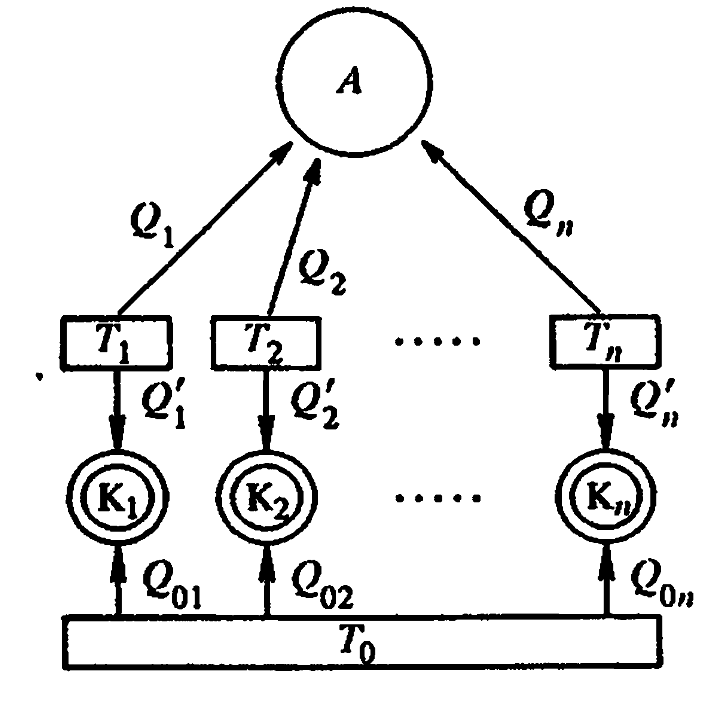
\includegraphics[width=50mm]{ris.png}
	\end{figure}
\end{minipage}
\begin{minipage}{115mm}
	Для i-ой машины за 1 цикл: $1+\dfrac{Q_i'}{Q_{oi}}=1-\dfrac{T_i}{T_o} \Leftrightarrow\dfrac{Q_{oi}}{T_o}+\dfrac{Q_i'}{T_i}=0$.\\
	Суммируя по i: $Q_o=\sum_iQ_{oi}=-T_o\sum_i\dfrac{Q_i'}{T_i}$\\
	$Q_o$ --- общее количество теплоты, отданное $R_o$. Объединим все $n$ циклов машин Карно с циклом A в один большой: $R_o$ отдал $Q_o$; $R_1$ отдал $Q_1+Q_1';\ldots\;R_n$ отдал $Q_n+Q_n'$. Совершена работа $A=Q_o+(Q_1+Q_1')+\ldots(Q_n+Q_n')$. В силу больших размеров $R_1,\ldots,R_n$ выберем в согласии с постулатом Томсона--Планка $Q_1',\ldots,Q_n'$ так, что \\
	$Q_i'+Q_i=0,\,i=\overline{1,n}\then$ все тепловые резервуары вернутся в исходное состояние, а $R_o$ отдаст $Q_o=T_o\sum_{i=1}^{n}\dfrac{Q_i}{T_i}$\\
\end{minipage}
Таким образом совершается круговой процесс, за который отдано $Q_o$ и совершена работа $A=Q_o$. Других изменений не произошло. Тогда $A\leqslant0$ из постулата Томсона--Планка, значит $Q_o\leqslant0$. Переходя к пределу бесконечно большого числа тепловых резервуаров $R_1,\ldots,R_n,\dots$, обменивающихся бесконечно малыми порциями тепла с A и $R_o$ получаем:
$$\oint\dfrac{\delta Q}{T}\leqslant0\text{ --- \textbf{неравенство Клаузиуса}}$$
$T$ --- температура теплового резервуара, с которым система в данным момент обменивается теплом. В квазистатическом цикле под $T$ можно понимать температуру окружающей среды, так как обе температуры одинаковы.\\
Квазистатический процесс обратим, следовательно справедливо $\oint\dfrac{\delta Q'}{T}\leqslant0$, где $\delta Q'$ --- элементарное количество теплоты, получаемое системой на отдельных участках процесса. Так как процесс идет через те же состояния, то $\delta Q=-\delta Q'\then\oint\dfrac{\delta Q}{T}\geqslant$0. А такое соотношение верно только тогда, когда $$\oint_\text{квазист.}\dfrac{\delta Q}{T}=0\text{ --- \textbf{равенство Клаузиуса}}$$

\begin{wrapfigure}{l}{30mm}
	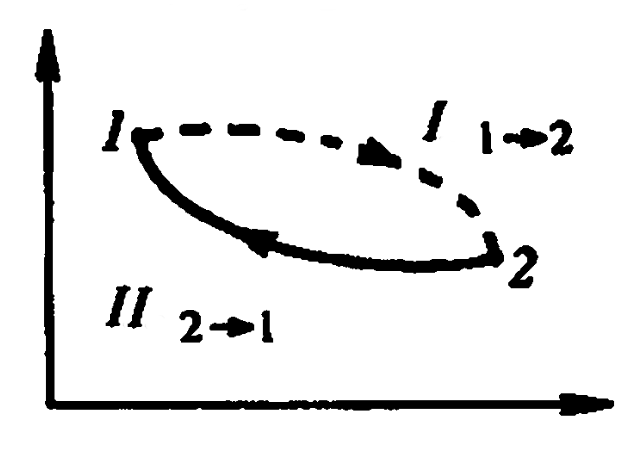
\includegraphics[width=30mm]{ris10.png}
\end{wrapfigure}
\paragraph{Энтропия.} Рассмотрим 2 способа перехода из 1 в 2, каждый из которых --- квазистатический процесс. Объединим их в круговой 1\RomanNumeralCaps{1}2\RomanNumeralCaps{2}1 и применим равенство Клаузиуса.
$$\int_{1\RomanNumeralCaps{1}2}\dfrac{\delta Q}{T} + \int_{2\RomanNumeralCaps{2}1}\dfrac{\delta Q}{T}=0\Leftrightarrow\int_{1\RomanNumeralCaps{1}2}\dfrac{\delta Q}{T}=\int_{1\RomanNumeralCaps{2}2}\dfrac{\delta Q}{T}\text{ --- приведенное количество теплоты.}$$
Таким образом приведенное количество теплоты, полученное системой при любом квазистатическом круговом процессе равно нулю \textbf{или} приведенное количество теплоты, полученное системой в квазистатическом процессе, не зависит от пути перехода, а определяется лишь начальным и конечным состояниями.\\
Отсюда: \textbf{энтропия} --- функция состояния системы, определенная с точностью до константы.
$$\Delta S \equiv \int_{1\rightarrow2}\dfrac{\delta Q}{T},\;\;dS=\left(\dfrac{\delta Q}{T}\right)_\text{кваз.}$$
\paragraph{Энтропия идеального газа.}
\textbf{Для идеального газа:} $$\delta Q=C_VdT+PdV=C_V(T)dT+R\dfrac{dV}{V}T\Leftrightarrow dS=\dfrac{\delta Q}{T}=\nu C_V(T)\dfrac{dT}{T}+\nu R\dfrac{dV}{V}$$
$$S=\int C_V(T)\dfrac{dT}{T}+R\int \dfrac{dV}{V}$$
Если $C_V$ не зависит от $T$, то $S=\nu[C_v\ln(T)+R\ln\left(V\right)]+const$. Всякий адиабатический процесс с $\delta Q=0\then dS=0\then S=const$.
\paragraph{Закон возрастания энтропии.} Энтропия адиабатически изолированной системы не может убывать, она либо растет, либо постоянна. 
Система может переходить из 1 в 2 необратимо по \RomanNumeralCaps{1}. Вернем ее квазистатически по какому-либо \RomanNumeralCaps{2}. Тогда
$\oint\dfrac{\delta Q}{T}=\int_\RomanNumeralCaps{1}\dfrac{\delta Q}{T}+\int_{\RomanNumeralCaps{2}}\dfrac{\delta Q}{T}\leqslant0$.
Так как $\int_{\RomanNumeralCaps{2}}\dfrac{\delta Q}{T}=S_1-S_2\then S_2-S_1\geqslant\int_{1\rightarrow2}\dfrac{\delta Q}{T}$. Если система адиабатически изолирована, то $\delta Q=0\then S_2\geqslant S_1$.


  
 \section{\normalsize  Термодинамические потенциалы. Метод получения соотношений Максвелла (соотношений взаимности). }
\paragraph{Термодинамические потенциалы.} \textbf{Термодинамические потенциалы} --- функции определенных наборов термодинамических параметров, позволяющие находить все термодинамические характеристики системы, как функции этих параметров.
\paragraph{Метод получения соотношений Максвелла (соотношений взаимности).} У Леши Шевцова он представлен на примере вывод одного из потенциалов. В Сивухине похожая ситуация, так что пока что опустим этот пункт, а в следующем билете вы увидите, что это за метод и в чем его суть.

   
 \section{\normalsize Свободная энергия Гельмгольца, термодинамический потенциал Гиббса. Уравнения Гиббса--Гельмгольца.}
\paragraph{Свободная энергия Гельмгольца.} $$\Psi=\Psi(T,V)=U-TS\then d\Psi=-PdV-SdT\then -S=\left(\dfrac{\partial \Psi}{\partial T}\right)_V,\;-P=\left(\dfrac{\partial\Psi}{\partial V}\right)_T\then$$ $$\then\dfrac{\partial^2 \Psi}{\partial V\partial T}=\dfrac{\partial^2 \Psi}{\partial T\partial V}\Leftrightarrow\dfrac{\partial}{\partial V}\left(\dfrac{\partial \Psi}{\partial T}\right)_V=\dfrac{\partial}{\partial T}\left(\dfrac{\partial \Psi}{\partial V}\right)_T\Leftrightarrow\underline{\left(\dfrac{\partial S}{\partial V}\right)_T=\left(\dfrac{\partial P}{\partial T}\right)_V}$$
Вот такой метод получения данных соотношений через двойное дифференцирование и называется \textbf{методом Максвелла}.
\paragraph{Термодинамический потенциал Гиббса.} $$\Phi=\Phi(T,P)=U-TS+PV\then d\Phi=VdP-SdT\then V =\chpr{\Phi}{P}{T},\;-S=\chpr{\Phi}{T}{P}\then$$
$$\then\vtchpr{T}{\Phi}{P}{T}=\vtchpr{P}{\Phi}{T}{P}\Leftrightarrow\underline{\chpr{V}{T}{P}=-\chpr{S}{P}{T}}$$
\paragraph{Уравнения Гиббса-Гельмгольца.} Из свободной энергии Гельмгольца $U = \Psi + TS$ подставим $S$ полученное при частном дифференцировании, тогда $U = \Psi -T\chpr{\Psi}{T}{V}$. Проведем аналогичные действия с термодинамическим потенциалом Гиббса: \\$I = \Phi - T\chpr{\Phi}{T}{P}$. Данные соотношения называются \textbf{Уравнениями Гиббса-Гельмгольца}

 
 \section{\normalsize  Внутренняя энергия как термодинамический потенциал. Связь производной $\Chpr{U}{V}{T}$с термическим уравнением состояния.}
\paragraph{Внутренняя энергия как термодинамический потенциал.} 
$$U = U(S,V) \then dU=TdS-PdV\then T=\chpr{U}{S}{V},\;-P=\chpr{U}{V}{S}\then$$
$$\then\vtchpr{V}{U}{S}{V}=\vtchpr{S}{U}{V}{S}\Leftrightarrow\underline{\chpr{T}{V}{S}=-\chpr{P}{S}{V}}$$
\paragraph{Связь производной $\Chpr{U}{V}{T}$с термическим уравнением состояния.}
$$dU=TdS-PdV\then\chpr{U}{V}{T}=T\chpr{S}{V}{T}-P=T\chpr{P}{T}{V}-P$$
Полученное соотношение устанавливает связь между калорическим и термическим уравнениями состояния.
   
 \section{\normalsize Разность $C_P-C_V$ для произвольной термодинамической системы.} 
$$CdT=dU+PdV=\chpr{U}{T}{V}dT+\left[P+\chpr{U}{V}{T}\right]dV$$
Полагая $C=C_P$:
$$C_P-C_V=\left[P+\chpr{U}{V}{T}\right]\chpr{V}{T}{P}$$
\text{воспользуемся соотношением из п. 13.2}
$$C_P-C_V=T\chpr{P}{T}{V}\chpr{V}{T}{P}=\left|\chpr{P}{T}{V}\chpr{T}{V}{P}\chpr{V}{P}{T}=-1\right|=-T\dfrac{\Chpr{V}{T}{P}^2}{\Chpr{V}{P}{T}}$$
Поскольку $\chpr{V}{P}{T}<0$, то $C_P-C_V>0$.
 
 \section{\normalsize Теплофизические свойства твердых тел. Адиабатическое растяжение упругого стержня.}
\paragraph{Теплофизические свойства твердых тел.} \textbf{Теплофизические свойства материала} -- свойства, характеризующие поведение этого материала при изменении температуры, как-либо: теплоемкость, теплопроводность, коэффициенты теплового расширения, температура плавления.
\paragraph{Адиабатическое растяжение упругого стержня.} \textbf{Уравнение состояния} --- $f~=~f(l,T)$. При $f=0$ $l(T,0)=l_0(1+\alpha(T-T_0))$, где $l_0=l(T_0,0)$, $\alpha$ --- коэффициент линейного температурного расширения. При $T=const$ согласно закону Гука: $$\dfrac{\Delta l}{l}=\dfrac{f}{ES_\perp}=\dfrac{l(T,f)-l(T,0)}{l(T,0)}\then f=ES_\perp\left(\dfrac{l}{l_0(1+\alpha[T-T_0])}-1\right)$$
В большинстве случаев тепловая деформация мала, $\alpha|T-T_0|\ll1\then$
$$\then f=ES_\perp\left(\dfrac{l}{l_0}(1-\alpha[T-T_0])-1\right)$$
Предположен, что стержень окружен адиабатической оболочкой. При квазистатической деформации $dS=\chpr{S}{T}{l}dT+\chpr{S}{l}{T}dl=0\Rightarrow dT=-\dfrac{\Chpr{S}{l}{T}}{\Chpr{S}{T}{l}}dl;\;\chpr{S}{T}{l}=\left(\dfrac{\delta Q}{\partial T}\right)_l~\dfrac{1}{T}~=~\dfrac{C_l}{T}$ \\
$$PdV=-\sigma d(S_\perp l)=-\sigma S_\perp dl=-fdl\Rightarrow dU=TdS+fdl$$
$$\Psi=U-TS,\,d\Psi=-SdT+fdl\Rightarrow -\chpr{S}{l}{T}=\chpr{f}{T}{l}\text{( по методу Максвелла)}$$
Откуда 
$$dT=\dfrac{T}{C_l}\chpr{f}{T}{l}dl$$
Используя $f:\,\Delta T=\int_{l_0}^{l}\dfrac{T}{C_l}\chpr{f}{T}{l}dl=-\dfrac{ES_\perp \alpha}{2C_ll_0}T(l^2-l_0^2)\simeq\underline{-\dfrac{ES_\perp\alpha}{C_l}T(l-l_0)}$\\
При адиабатическом растяжении ($l>l_0$) температура стержня понижается из-за совершения работы против внутренних сил притяжения молекул. Для идеального стержня ($E=const$):
$$U_\text{деф.}=V\dfrac{E\varepsilon^2}{2}=\Psi_\text{деф.}$$
Внутренняя энергия деформации совпадает со свободной энергией и явно не зависит от температуры.

 
 \section{\normalsize Фазовые переходы первого рода. Уравнение Клапейрона--Клаузиуса. Фазовое равновесие «жидкость--пар». Критическая точка.}
\paragraph{Фазовые переходы первого рода.} \textbf{Фаза} --- макроскопическая физическая однородная часть вещества, отделённая от остальных частей системы границами раздела, так что она может быть извлечена из системы механическим путём.\\
\textbf{Фазовый переход} --- переход вещества из одной фазы в другую при изменении внешних условий (температуры, давления, полей) при подводе или отводе тепла и т.д. \\
Величины, пропорциональные объёму подсистемы называются \textbf{экстенсивными} ($V,U,S$), а не зависящие от объёма выделенной подсистемыы --- \textbf{интенсивными} ($T,P,\rho$).\\
Фазовые превращения, при которых первые производные удельного термодинамического потенциала $\varphi(T,P)$ меняются скочкообразно называются \textbf{фазовыми переходами первого рода}\\
$v=\chpr{\varphi}{P}{T},\,s=-\chpr{\varphi}{T}{P}\Rightarrow$ скачкообразно меняется плотность ($\rho\simeq\frac{1}{v})$. Отлична от нуля теплота фазового перехода $q_{12}=T(s_2-s_1)$. \\
Плавление, испарение, возгонка, кристаллизация сопровождаются выделением или поглощением тепла, поэтому относятся к Ф.П. \RomanNumeralCaps{1} рода.
\paragraph{Уравнение Клапейрона--Клаузиуса.} Условия равновесия системы: 
\begin{enumerate}[1)]
	\item $P=const$ --- условие механического равновесия;
	\item $T=const$ --- условие теплового равновесия;
	\item $\varphi=const$ --- условие фазового перехода.
\end{enumerate}
Обоснование 3) : \\
	Рассмотрим двух фазную сиситему в жесткой адиабатической оболочке. Проведем в системе некий бесконечно малый процесс, в холе которого $T=const,\,P=const$ в обоих подсистемах и равны между собой, тогда:\\ $dU_1=TdS_1-PdV_1+\varphi_1dN_1;\;$\\$dU_2=TdS_2-PdV_2+\varphi_2dN_2$;\\
	Полная энтропия системы $S=S_1+S_2$, а в следствие изолированности $dU_1=-dU_2\Rightarrow\\\Rightarrow TdS=(\varphi_1-\varphi_2)dN_2$.В состоянии термодинамического равновесия энтропия максимальная, значит $dS=0\Rightarrow\varphi_1=\varphi_2$\\
    $d\varphi_1=-s_1dT+v_1dP,\quad d\varphi_2=-s_2dT+v_2dP,\quad\varphi_1=\varphi_2\Rightarrow d\varphi_1=d\varphi_2\Rightarrow$\\
    $\Rightarrow(s_2-s_1)dT=(v_2-v_1)dP\Leftrightarrow\dfrac{dP}{dT}=\dfrac{s_2-s_1}{v_2-v_1},\quad q_{12}=T(v_2-v_1)$ --- теплота фаз перехода в расчете на 1 частицу $\then \dfrac{dP}{dT}=\dfrac{q_{12}}{T(v_2-v_1)}$ --- \textbf{Уравнение Клапейрона--Клаузиуса}.
\paragraph{Фазовое равновесие «жидкость--пар».}$\;$\\
\begin{minipage}{75mm}
	\begin{figure}[H]
		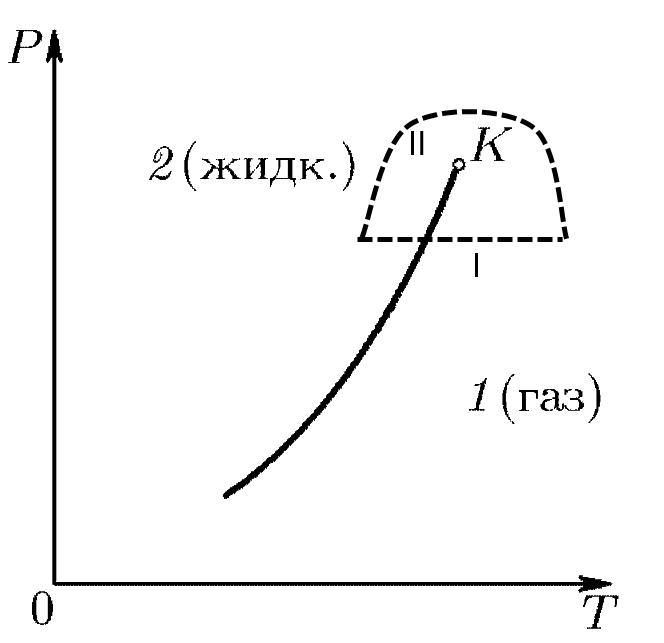
\includegraphics[width=65mm]{Klap.png}
	\end{figure}
\end{minipage}
\begin{minipage}{100mm}
	 Примем $q_{12}=q=const\Rightarrow\dfrac{dP}{dT}=\dfrac{q}{T(v_1-v_2)}$\\
	 Так как $v_1\gg v_2$:\\
	 $\simeq\left.\dfrac{q}{Tv_1}\right|_{Pv_1=kT}=\dfrac{q}{kT^2}P\Leftrightarrow\int_{P_0}^{P}=\dfrac{dP}{P}=\dfrac{q}{k}\int_{T_0}^{T}\dfrac{dT}{T^2}\Rightarrow\\
	 \Rightarrow P=P_0exp\left(\dfrac{q}{kT_0}-\dfrac{q}{kT}\right), P(T_0)=P_0$\\
	 \textbf{Критическая точка(К)} --- точка, в которой обрывается кривая фазового равновесия и исчезает разница между фазами. При наличии К всегда есть путь, в каждый момент которого вещество однородно, т.е. не возникает граница раздела.
\end{minipage}
 I --- пересекая кривую фазового равновесия (с образованием двухфазовой системы)\\
II --- в обход К (сохраняя пространственную однородность)\\
Для воды: $T_\text{кр.}=647.3\text{ К, }P_\text{кр.}=22.12\text{ МПа}$
  
 \section{\normalsize Диаграмма фазового равновесия «твёрдое тело--жидкость--пар». Тройная точка.}
\paragraph{Диаграмма фазового равновесия «твёрдое тело--жидкость--пар».}$\;$\\
\begin{minipage}{75mm}
	\begin{figure}[H]
		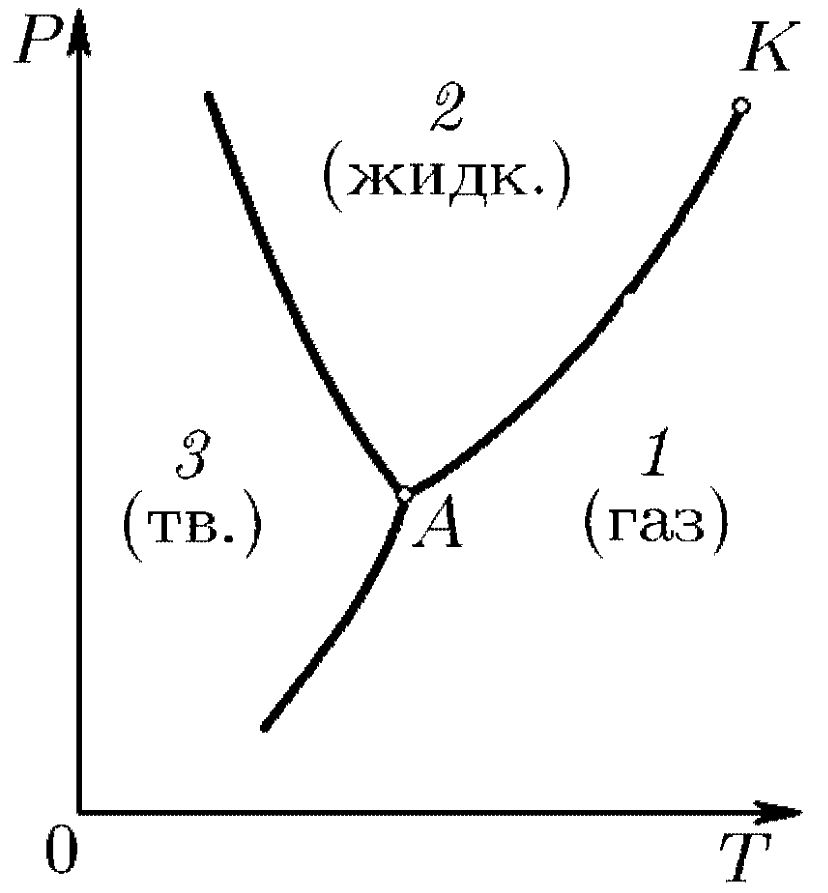
\includegraphics[width=65mm]{ris17.png}
	\end{figure}
\end{minipage}
\begin{minipage}{100mm}
	Рассмотрим трех фазную систему. Для равновесия необходимо:
	\begin{enumerate}[(1)]
		\item $\varphi_1(P,T)=\varphi_2(P,T)$ --- кривая испарения 12
		\item $\varphi_2(P,T)=\varphi_3(P,T)$ --- кривая плавления 23
		\item $\varphi_1(P,T)=\varphi_3(P,T)$ --- кривая возгонки 31
	\end{enumerate}
	Все они пересекаются в т.А
\end{minipage}
\paragraph{Тройная точка.}
Точка А называется \textbf{тройной точкой}, три фазы могут находится в равновесии друг с другом, лишь в этой точке, имеющей конкретный параметры. В малой окрестности тройной точки можно провести круговой изотермический процесс, для которого справедливо
$$\oint\dfrac{\delta Q}{T}=0\underset{T=const}{\longmapsto}\oint\delta Q \Rightarrow q_\text{13}=q_\text{32}+q_\text{21}$$

   
 \section{\normalsize Зависимость теплоты фазового перехода от температуры.}
$$q=T(S_2-S_1)\text{ --- удельная теплота фазового превращения.}$$
    
 \section{\normalsize Уравнение Ван-дер-Ваальса как модель неидеального газа. Изотермы газа Ван-дер-Ваальса. Критические параметры. Приведённое уравнение Ван-дер-Ваальса, закон соответственных состояний.}
\paragraph{Уравнение Ван-дер-Ваальса.}
$$\left(P+\dfrac{a\nu^2}{V^2}\right)\left(V-\nu b\right)=RT$$

\begin{wrapfigure}{R}{5cm}
	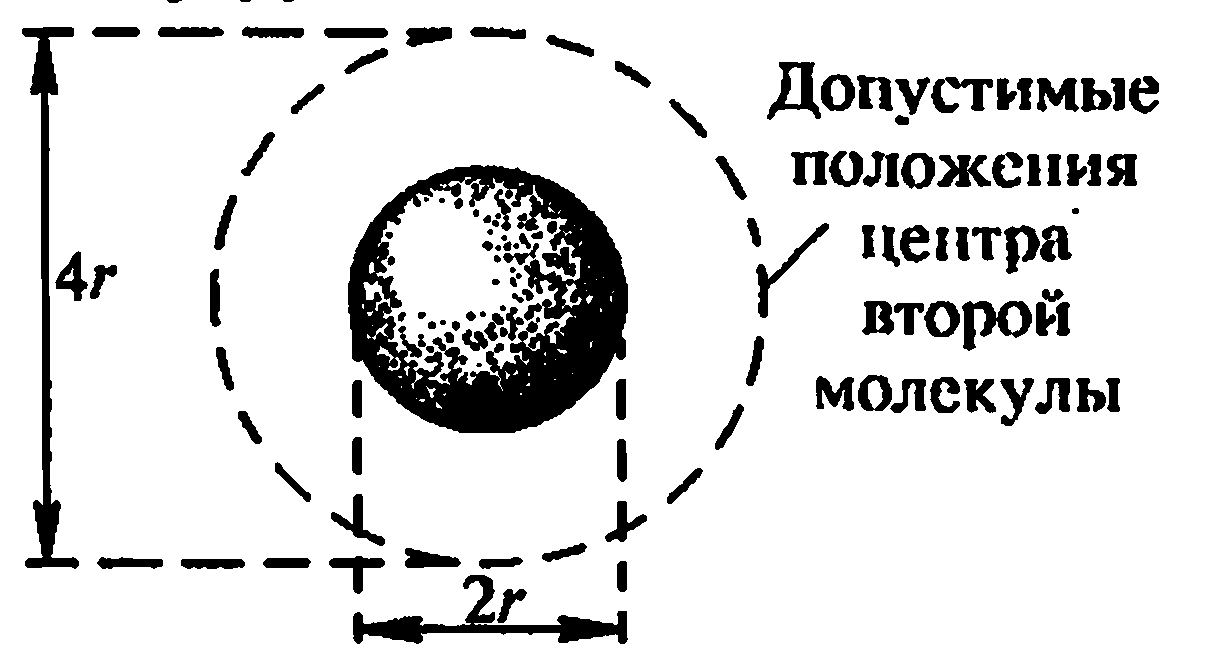
\includegraphics[width=65mm]{ris19.png}
	\caption{Учет конечности размеров молекул}
\end{wrapfigure}
Выведем его, основываясь на $PV=\nu RT$:\\
Во-первых, учтем размеры молекул: \\$\dfrac{4}{3}\pi(2r)^3=8\cdot\dfrac{4}{3}\pi r^3$ --- недоступный объем для второй частицы $\Rightarrow$ в расчете на 1 молекулу $$\dfrac{1}{2}(8\cdot\dfrac{4}{3}\pi r^3)=4V_0$$
где $V_0=4\pi r^3/3$ --- объем одной молекулы. 
В результате объем, разрещенный для движения молекул, cоставит
$$V_\text{доп.} =V-\nu b,\quad$$
$$ b\simeq4\cdot\text{(объем молекулы в одном моле)}=4N_AV_0$$
Во-вторых, учтем, что молекулы притягиваются другк другу. Одним из механизмов такого притяжения может быть перераспределение зарядов и образование диполей (см. рис 2).

\begin{wrapfigure}{l}{4cm}
	\label{dipol}
	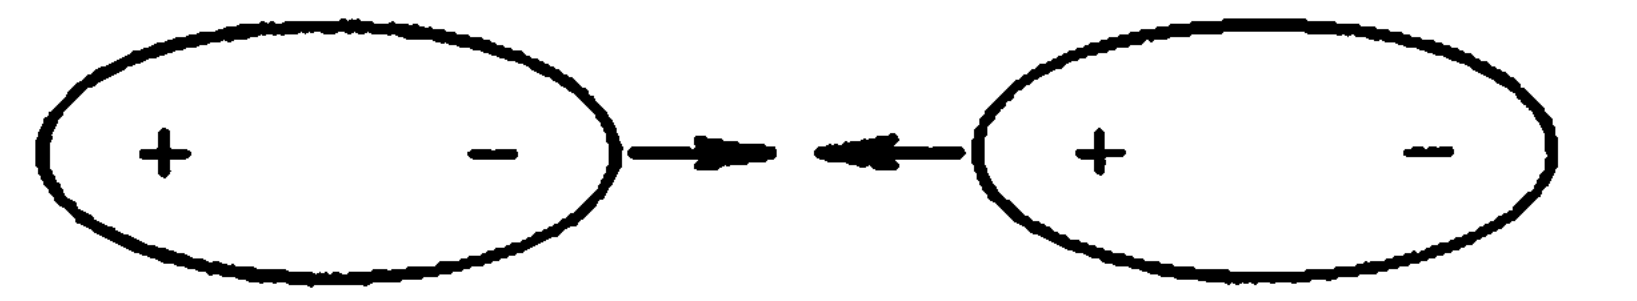
\includegraphics[width=40mm]{ris19_2.png}
	\caption{\small Молекулы--диполи притягиваются друг к другу}
\end{wrapfigure}
Давление газа определяется столкновениями молекул со стенкой. Сила, действующая на молекулу у стенки со стороны газа $\sim n$, где $n$ --- число частиц. Частота соударений $\sim n$, значит давление уменьша-
ется на $\Delta P\sim n^2$. Переходя от плотности $n$ к объему $V$ по формуле $n=\dfrac{\nu N_A}{V}$, мы можем записать поправку к давлению в виде $\Delta P=a_1n^2=a(\nu/V)^2.$ Окончательно это даёт
$$\left(P+\dfrac{a\nu^2}{V^2}\right)\left(V-\nu b\right)=RT$$
Величины $a$ и $b$ называется параметрами Ван-дер-Ваадбся. Параметре $a$ учитывает притяжение, а $b$ --- отталкивание молекул.
\paragraph{Изотермы газа Ван-дер-Ваальса. Критические параметры.}

\begin{wrapfigure}{r}{8cm}
	\label{VdV}
	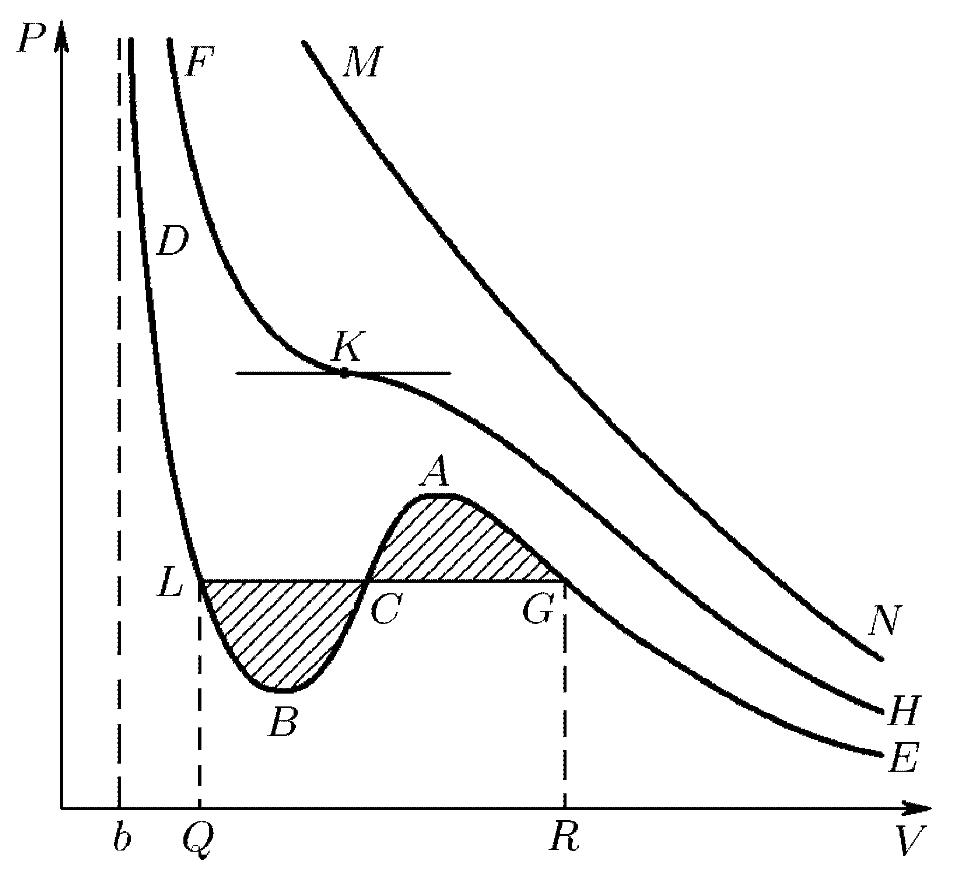
\includegraphics[width=80mm]{ris19_3.png}
	\caption{Изотермы Ван-дер-Ваальса}
\end{wrapfigure}
Уравнение Ван-дер-Ваальса: $$PV^3-(RT+\\+Pb)V^2+aV-ab=0$$ имеет один или три корня. В случае 1 это изотерма MN, а трех --- три пересечегтя в точках A, C, E изотермы LABCDEG. При некоторой $T$ $V_1=V_2=V_3$. Такая температура называется \textbf{критической} (изотерма FKH). Для нахлждения критиечских давления, температуры и объема воспользуемся уравнением: $P_\text{к.}~(V~-~V_\text{к.})^3~=~0$\\

\begin{equation*}
\begin{cases}
P_\text{к.}V_\text{к.}^3=ab\\
3P_\text{к.}V_\text{к.}^2=a\\
3P_\text{к.}V_\text{к.}=RT_\text{к.}+P_\text{к.}b
\end{cases}
\Leftrightarrow
\begin{cases}
P_\text{к.}=\dfrac{a}{27b^2}\\
V_\text{к.}=3b\\
T_\text{к.}=\dfrac{8a}{27Rb}
\end{cases}
\end{equation*}
\paragraph{Приведённое уравнение Ван-дер-Ваальса} $\varphi=\dfrac{V}{V_\text{к.}},\quad\pi=\dfrac{P}{P_\text{к.}},\quad\tau=\dfrac{T}{T_\text{к.}}$ --- приведённые параметры. Тогда $V~=~3b\varphi,\quad P~=~\dfrac{a\pi}{27b^2},\\T~=~\dfrac{8a}{27Rb}~\tau\Rightarrow$ \textbf{приведённое уравнение Ван-дер-Ваальса}:
\begin{equation*}
\left(\pi+\dfrac{3}{\varphi^2}\right)(\varphi-1/3)=8/3\tau
\end{equation*}
\paragraph{Закон соответственных состояний.}Уравнение Ван-дер-Ваальса содержит только 3 параметра: $a,\,b,\,R$. Всякое уравнение, обладающее этим свойством, записанное в переменных $\varphi,\,\pi,\,\tau$ должно быть также одинаковым для всех веществ. Это положение есть \textbf{закон соответственных состояний}.\\
\textbf{Соответственными} называют состояния разных веществ, которые имеют одинаковые $\varphi,\,\pi,\,\tau$. Следовательно: если для различных веществ из трех параметров $\varphi,\,\pi,\,\tau$ совпадают значения каких-либо двух, то совпадут и третьи.
    
 \section{\normalsize Метастабильные состояния: переохлаждённый пар, перегретая жидкость. Устойчивость состояний. Правило Максвелла.}
\paragraph{Метастабильные состояния: переохлаждённый пар, перегретая жидкость. Устойчивость состояний.} При специальных условия могут быть реализованы участки AG --- перенасыщенный пар и LB --- перегретая жидкость (см. рис. 3). Эти состояния называют \textbf{метастабильными}. Каждое существует, пока его менее устойчивая фаза не граничит с другой --- более устойчивой. Например, перенасыщенный пар переходит в насыщенный, если в него попадёт капля воды.
\paragraph{Правило Максвелла.}Положение горизонтального участка определяется с помощью равенства Клазиуса $\oint\dfrac{\delta Q}{T}=0$. Из G в L можно перейти двумя путями: по GCL двухфазного состояния и по теоретической изотерме физически однородного вещества GACBL, содержащей неустойчивый участок ACB. Применим равенство Клаузиуса к квазистатическому круговому процессу GCLBCAG: $T=const\Rightarrow\oint\delta Q=0$, кроме того $\delta Q~=~dU~+~PV,\quad \\\oint dU=0\Rightarrow\oint PdV=0$ или $\int_{\text{GCL}}PdV+\int_{\text{LBCAG}}PdV=0$ или $\int_\text{LCG}PdV=\int_\text{LBCAG}PdV$\\
Значит площади QLGR и QLBCAGR равны, значит LG надо проводить так, чтобы $$S_\text{LBC}=S_\text{CAG}$$ Это и есть \textbf{правило Максвелла.}

     
 \section{\normalsize Внутренняя энергия и энтропия газа Ван-дер-Ваальса. Равновесное и неравновесное расширение газа Ван-дер-Ваальса в теплоизолированном сосуде.
}
\paragraph{Внутренняя энергия и энтропия газа Ван-дер-Ваальса.} Рассмотрим $U=U(T,V)$, тогда $dU=\chpr{U}{T}{V}dT+\chpr{U}{V}{T}dV=C_VdT+\left(T\chpr{P}{T}{V}-P\right)dV$. Для $\nu$ = 1 моль, предполагая $C_V=const,\ dU=C_VdT+\dfrac{a}{V^2}dV$
$$U=C_VT-\dfrac{a}{V}$$
С ростом объема и, следовательно, расстояния между молекулами (при $T=const$) внутренняя энергия газа растет.\\
Рассмотрим $S=S(T,V)$, тогда $dS=\chpr{S}{T}{V}dT+\chpr{S}{V}{T}dV=\dfrac{C_V}{T}dT+\chpr{P}{T}{V}dV$. Для $\nu=1$ моль, $C_V=const,\ dS=\dfrac{C_V}{T}dT+\dfrac{R}{V-b}dV$ 
$$S=S_0+C_V\ln\left(\dfrac{T}{T_0}\right)+R\ln\left(\dfrac{V-b}{V_0-b}\right)$$
\paragraph{Равновесное и неравновесное расширение газа Ван-дер-Ваальса в теплоизолированном сосуде.} Рассмотри \textbf{свободное расширение газа в вакуум.} Пусть в начальный момент газ Ван-дер-Ваальса находился в сосуде, занимая в нем объем $V$. После удаления перегородки газ получил возможность свободно расшириться до объема $V_2(V_2>V_1)$. Считая, что сосуд окружен теплоизолированной оболочкой найдем $\Delta T$ после установления равновесия. Поскольку $\delta Q=0$ и $\delta A=0$, то $dU=0$, а для газа Ван-дер-Ваальса\\ $U_{1,2}=C_VT_{1,2}-\dfrac{a}{V_{1,2}}\Rightarrow\Delta T=T_2-T_1=-\dfrac{a}{C_V}\left(\dfrac{1}{V_1}-\dfrac{1}{V_2}\right)<0$ значит газ в данном процессе \textbf{охлаждается}.\\
При расширении газа работа совершается против сил притяжения молекул. Эта работа производится за счет кинетической энергии и, значит, сопровождается охлаждением газа

      
 \section{\normalsize Эффект Джоуля--Томсона (дифференциальный и интегральный). Температура инверсии.} 
\paragraph{Дифференциальный эффект Джоуля--Томсона.} Рассмотрим процесс Джоуля--Томсона: адиабатическое стационарное течение газа через пористую перегородку, под действием разности давлений

\begin{wrapfigure}{L}{7cm}
	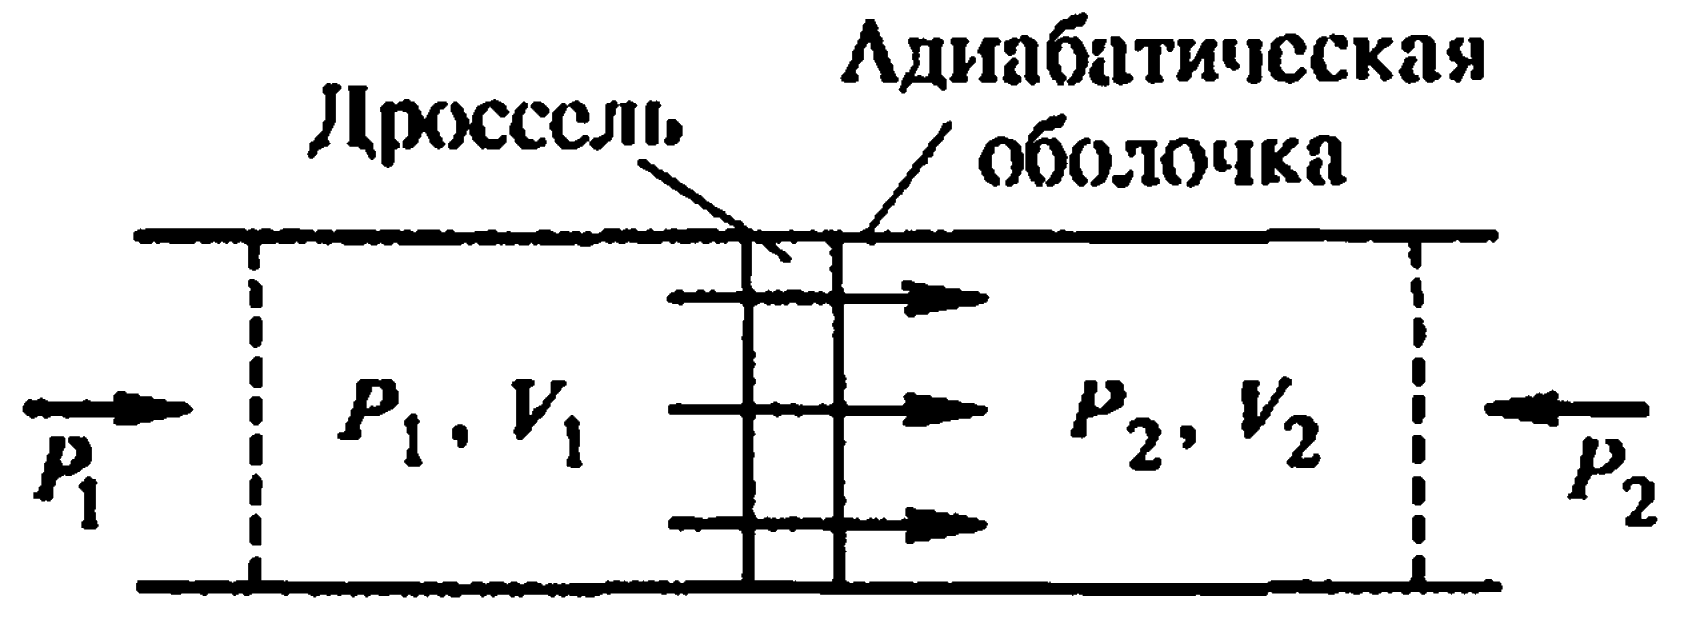
\includegraphics[width=70mm]{ris22_1.png}
\end{wrapfigure}
по разные стороны от пробки. Изменение температуры в этом процессе --- \textbf{эффект Джоуля-Томсона}. Течение медленное, следовательно можно пренебречь кинетической энергией. Тогда по первому началу термодинамики $Q=0\Rightarrow\\0=\Delta U+A=U_2-U_1+P_2V_2-P_1V_1=I_2-I_1\Leftrightarrow I_1=I_2$. В процессе Джоуля--Томсона $I=const$.\\
Пусть теперь по разные стороны от перегородки разность давлений мала. Найдем $\Delta T:$ $$\Delta I = \chpr{I}{T}{P}\Delta T+\chpr{I}{P}{T}\Delta P=0\Rightarrow\chpr{I}{T}{P}=C_P,\ \chpr{I}{P}{T}=V-T\chpr{V}{T}{P}\Rightarrow$$
$$\Rightarrow\left(\dfrac{\Delta T}{\Delta P}\right)_I=\dfrac{T\Chpr{V}{T}{P}-V}{C_P}$$
Если газ идеальный, то $V=\dfrac{RT}{P},\ T\chpr{V}{T}{P}=V\Rightarrow\Delta T=0$, то есть для идеальных газов эффект Джоуля--Томсона не имеет места. Повышение или понижение температуры реального газа при протекании через пробку при малых $\Delta T$ и $\Delta P$ $\left(\text{для замены их отношения на } \Chpr{T}{P}{I}\right)$ называется \textbf{дифференциальным эффектом Джоуля--Томсона}.\\
Так как течение происходит от большего давления к меньшему, то $\Delta P<0$, значит если $\frac{\Delta T}{\Delta P}>0$, то эффекто Джоуля--Томсона \textbf{положительный}, а если соответственно $\frac{\Delta T}{\Delta P}<0$ --- \textbf{отрицательный}.

\begin{wrapfigure}{R}{4cm}
	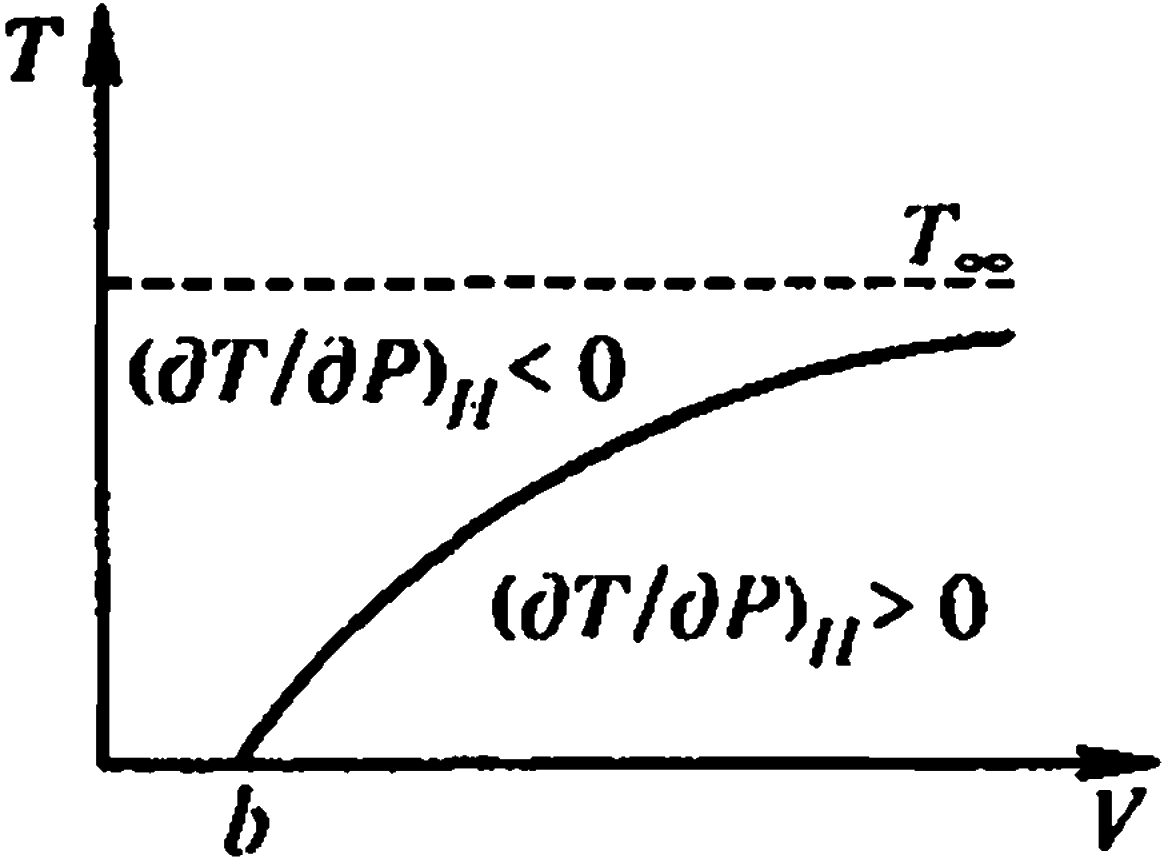
\includegraphics[width=40mm]{ris22_2.png}
\end{wrapfigure}
Вычисляя $\chpr{V}{T}{P}=\dfrac{-\Chpr{P}{T}{V}}{\Chpr{P}{V}{T}}$ из уравнения Ван-дер-Ваальса получаем:
$$\dfrac{\Delta T}{\Delta P}=-\dfrac{T\Chpr{P}{T}{V}+V\Chpr{P}{V}{T}}{C_P\Chpr{P}{V}{T}}=\dfrac{\frac{bRT}{(V-b)^2}-\frac{2a}{V^2}}{C_P\Chpr{P}{V}{T}}$$
\paragraph{Температура инверсии.} Пояснение к графику: $T_\infty\equiv T_i,\ H\equiv I$. В случае разреженного газа можно отбросить малые поправки $a$ и $b$ высших порядков $\Rightarrow\dfrac{\Delta T}{\Delta P}=\dfrac{\frac{2a}{RT}-b}{C_P}$. При $T_i=\dfrac{2a}{RB}=\dfrac{27}{4}T_\text{кр.}$ --- температуре инверсии дифференциального эффекта Джоуля--Томсона  $\Delta T=0$. Газ ниже этой температуры охлаждается, выше --- нагревается в процессе Джоуля--Томсона. \\
\paragraph{Интегральный эффект Джоуля--Томсона.} Пусть теперь по разные стороны от перегородки $\Delta P$ велика, тогда велика и $\Delta T$. Тогда мы имеем дело с \textbf{интегральным законом Джоуля--Томсона.}
\begin{equation}
T_2-T_1=\int_{P_1}^{P_2}\chpr{T}{P}{I}dP=\int_{P_1}^{P_2}\dfrac{T\Chpr{V}{T}{P}-V}{C_P}dP
\label{ur22}
\end{equation}
Если во всем диапазоне давлений дифференциального эффекта Джоуля--Томсона положительный, то и интегральный будет положительным. Максимальное охлаждение из начального состояния $T_1,\ P_1$: 
$$\dfrac{d}{dP_1}(T_2-T_1)=\dfrac{dT_2}{dP_1}=-\chpr{T}{P}{I}=0\text{ --- условие максимума записанное при }P=P_1,\ T=T_1$$
Но $\chpr{T}{P}{I}=0$ --- уравнение кривой инверсии дифференциального эффекта Джоуля--Томсона, следовательно, для максимального охлаждения  нужна точка на кривой инверсии дифференциального эффекта Джоуля--Томсона.\\
Формула (\ref{ur22}) интегрируется до конца в случае, когда в начальном состоянии газ под высоким давлением, а после прохода через вентиль его можно рассматривать как идеальный.
$$I_1=I_2\Leftrightarrow\int_{T_0}^{T_1}C_vTdT-\dfrac{a}{V_1}+P_1V_1=\int_{T_0}^{T_2}C_VTdT-\dfrac{a}{V_2}+P_2V_2\ \underset{\tfrac{a}{V_2}\rightarrow0}{\longrightarrow}\int_{T_2}^{T_1}C_VTdT-\dfrac{a}{V_1}+P_1V_1=RT_2$$
$$\overline{C_V}(T_1-T_2)-\dfrac{2a}{V_1}+\dfrac{RT_1V_1}{V_1-b}=RT_2,$$
где $\overline{C_V}$ --- средняя теплоемкость при $V=const$ в диапазоне $T_1\leftrightarrow T_2$. В итоге получим:


\begin{wrapfigure}{R}{52mm}
	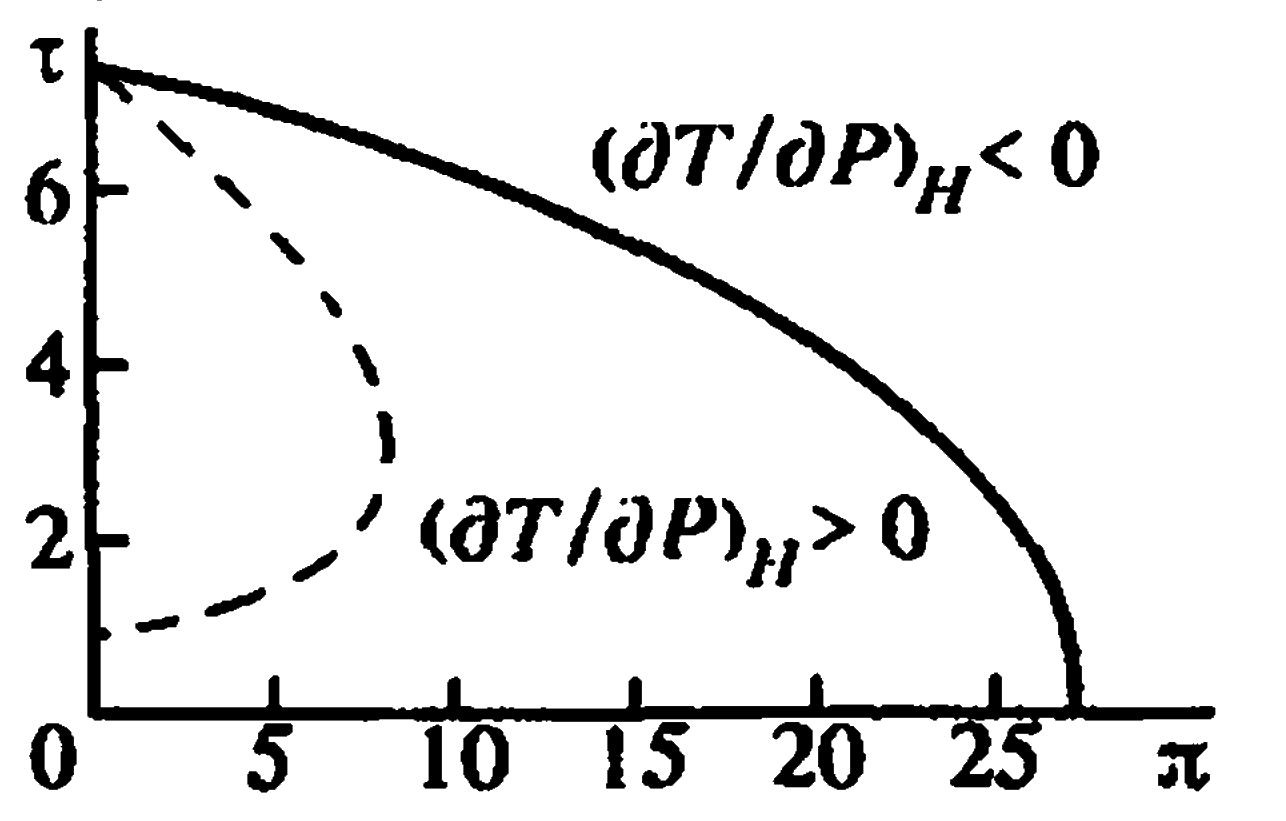
\includegraphics[width=50mm]{ris22_3.png}
	\caption{штрих. линия - кривая инверсии диф. эффекта}
\end{wrapfigure}
$$T_2-T_1=\dfrac{1}{R+\overline{C_V}}\left(\dfrac{RbT_1}{V_1-b}-\dfrac{2a}{V_1}\right)$$
Так как знаменатель положительный, то знак эффекта определяется знаком числителя.
\begin{enumerate}
	\item $T_1<\dfrac{2a}{Rb}\dfrac{V_1-b}{V_1}$ --- эффект положительный (охлаждение)
	\item $T_1>\dfrac{2a}{Rb}\dfrac{V_1-b}{V_1}$ --- эффект отрицательный (нагревание)
	\item $T_1=\dfrac{2a}{Rb}\dfrac{V_1-b}{V_1}$ --- температура инверсии интегрального эффекта Джоуля--Томсона
\end{enumerate}
$\tau=27/4\dfrac{\varphi-1/3}{\varphi}$ --- в приведенном виде, $\pi=27-16/27\tau^2\Leftrightarrow\tau=3/4\sqrt{81-3\pi}$

      
 \section{\normalsize Поверхностное натяжение: коэффициент поверхностного натяжения, краевой угол, смачивание и несмачивание. Формула Лапласа. Свободная энергия и внутренняя энергия поверхности.}
\paragraph{Поверхностное натяжение: коэффициент поверхностного натяжения, краевой угол, смачивание и несмачивание.} Работа, которую нужно затратить, чтобы изотермически и квазистатически увеличить поверхность жидкости на единицу при сохранении её объема неизменным называется \textbf{поверхностным натяжением жидкости.}

\begin{wrapfigure}{L}{3cm}
	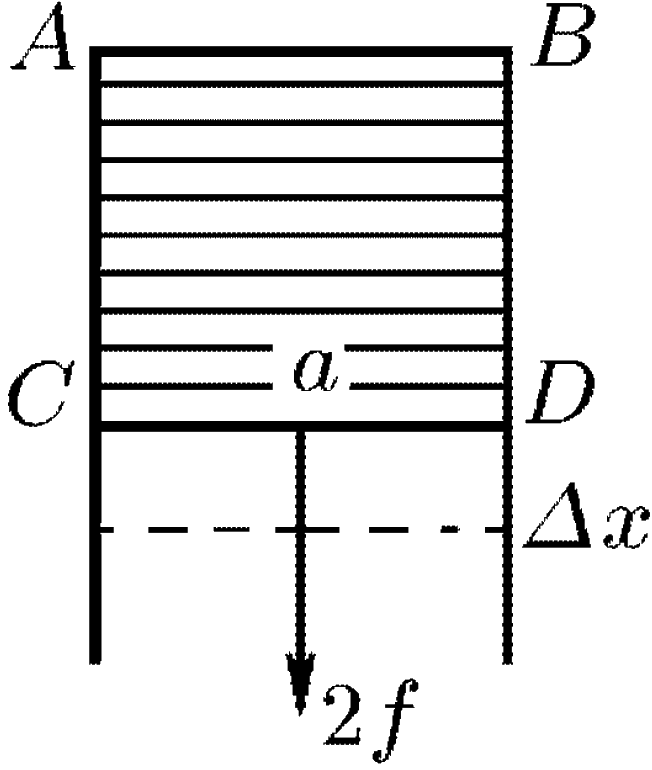
\includegraphics[width=30mm]{ris23_1.png}
\end{wrapfigure}
$$\sigma\equiv\dfrac{A}{\text{П}}\textbf{ --- коэффициент поверхностного натяжение, }$$
где $\text{П}\text{ --- площадь поверхности жидкости.}$ В изотермическом процессе работа идет на изменение $\Psi=\Psi_\text{об.}+\Psi_\text{пов.}$, где $\Psi_\text{об.}$ --- объемная энергия. $\Psi_\text{об.}\sim U$, а поверхностная энергия $\Psi_\text{пов.} =\sigma\text{П}$.
Пленка состоит из двух простых, значит $\delta A=2fdx$.
$$\sigma = \left(\dfrac{\delta A}{d\text{П}}\right)_T=\dfrac{2fdx}{2adx}=\dfrac{f}{a}$$
\begin{minipage}{55mm}
	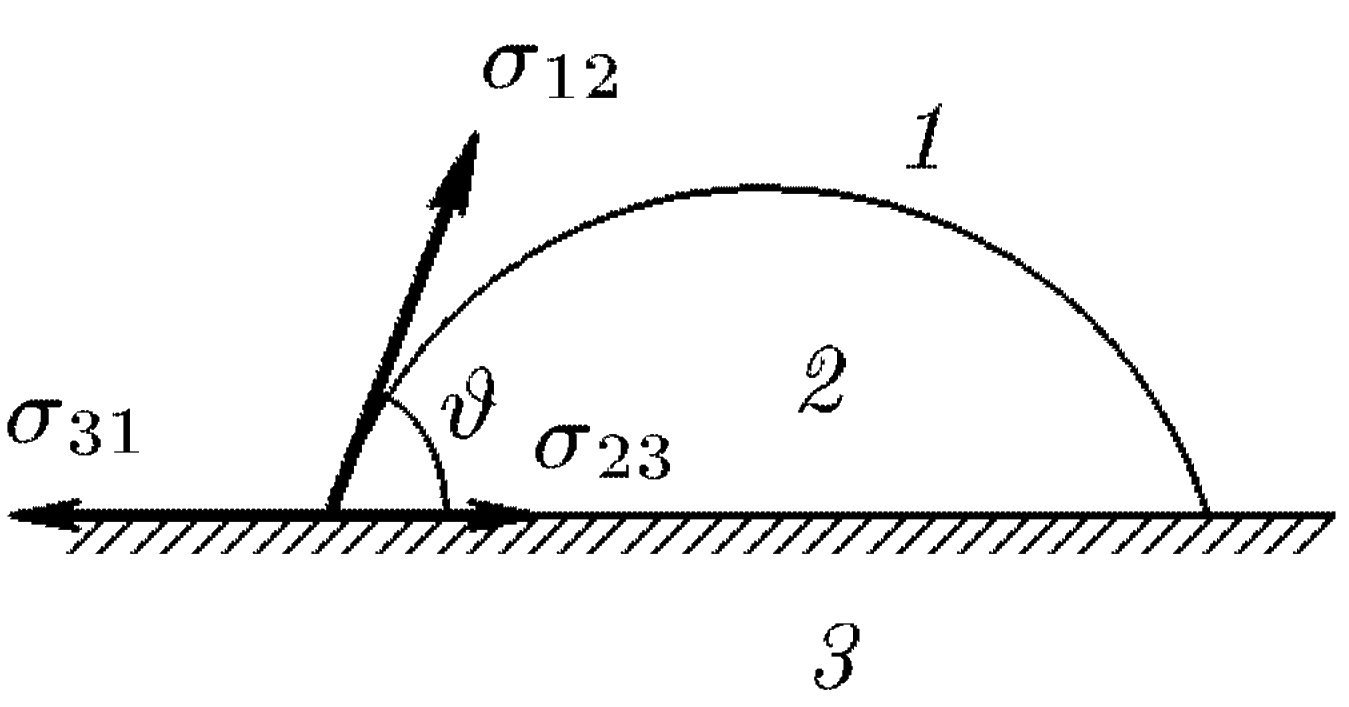
\includegraphics[width=50mm]{ris23_2.png}\\[-1cm] \center{a)}
\end{minipage}
\begin{minipage}{40mm}
	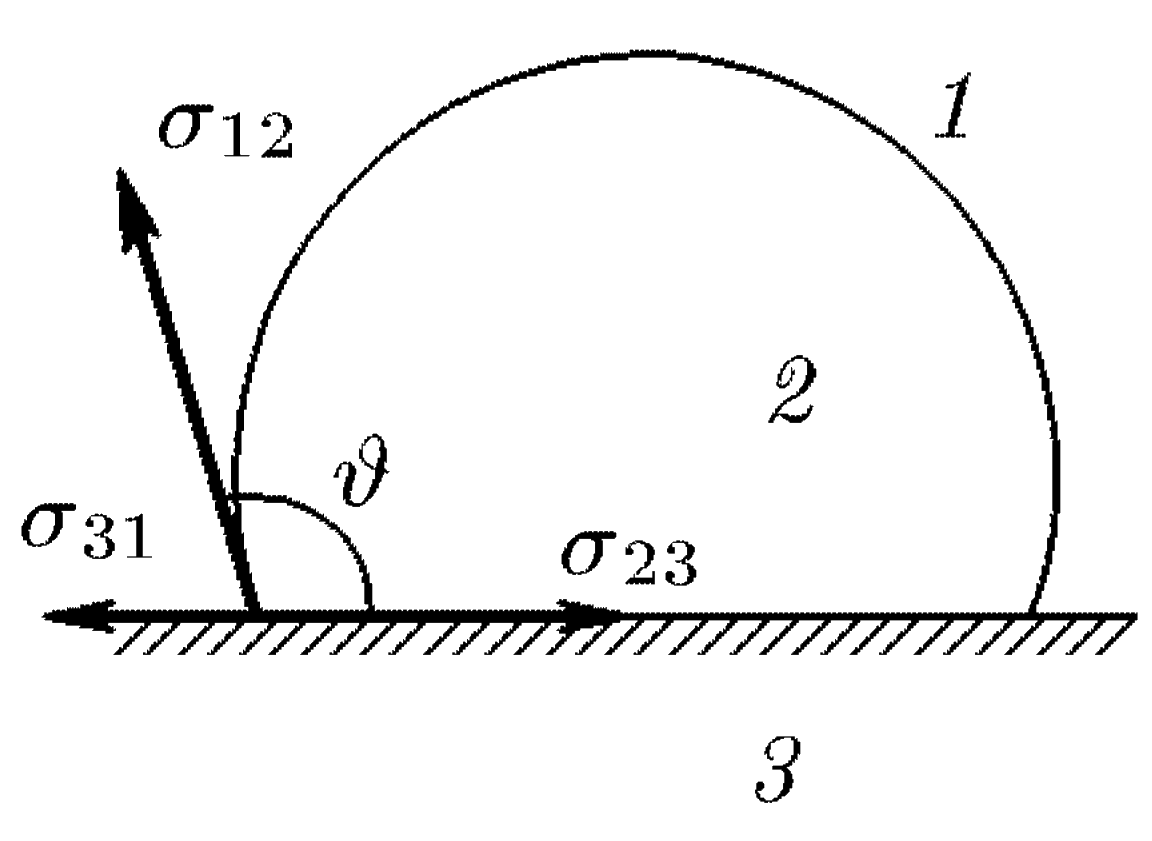
\includegraphics[width=35mm]{ris23_3.png} \\[-1cm] \center{б)}
\end{minipage}
\begin{minipage}{80mm}
	Равновесие: $\sigma_{31}+\sigma_{23}+\sigma_{12}cos\vartheta=0$, \\$\vartheta$ --- \textbf{краевой угол}..\\
	$\dfrac{\sigma_{13}-\sigma_{23}}{\sigma_{12}}>1$ --- \textbf{полное смачивание};\\
	$\dfrac{\sigma_{13}-\sigma_{23}}{\sigma_{12}}<-1$ --- \textbf{полное смачивание};
\end{minipage}
Также если $0<\vartheta<\pi/2$, то имеет место \textbf{частичное смачивание}, а при $\pi/2<\vartheta<\pi$ --- \textbf{частичное не смачивание}.\\[0.5cm]
\begin{minipage}{55mm}
	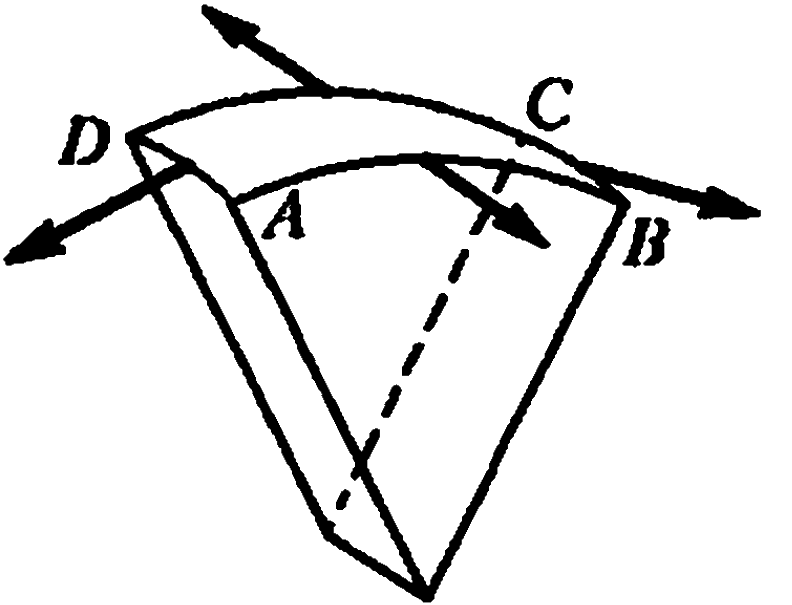
\includegraphics[width=50mm]{ris23_4.png}
	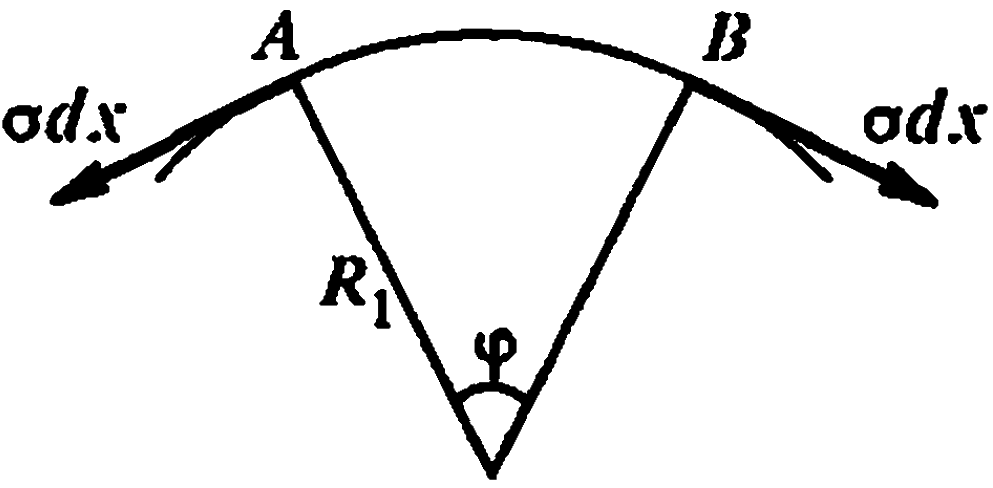
\includegraphics[width=50mm]{ris23_5.png}
\end{minipage}
\begin{minipage}{115mm}
	\paragraph{Формула Лапласа.}
	AD=$dx$, AB=$dy$ --- стороны прямоугольника, выделенного на кривой поверхности. Равнодействующая сил, приложенных к AD и BC направленна по радиусу и равна \\
	$dF_1=2\sigma dx\sin \varphi/2\simeq\sigma\varphi dx$, $\varphi=\dfrac{\text{AB}}{R_1}=\dfrac{dy}{R_1}\Rightarrow\\
	\Rightarrow dF_1=\dfrac{\sigma}{R_1}dx=\dfrac{\sigma}{R_1}d\text{П};
	\quad dF_2=\dfrac{\sigma}{R_2}d\text{П};\quad
	\\dF=dF_1+dF_2=\sigma\left(R_1^{-1}+R_2^{-1}\right)d\text{П}\Rightarrow$ $$P_2-P_1=\sigma\left(R_1^{-1}+R_2^{-1}\right)\textbf{ --- формула Лапласа}$$
	Для сферической поверхности: $\Delta p=\dfrac{2\sigma}{R}$, а для мыльного пузыря --- $\Delta P = (2\sigma)\dfrac{2}{R}=\dfrac{4\sigma}{R}$
\end{minipage}
\paragraph{Свободная энергия и внутренняя энергия поверхности.} По первому началу термодинамики: $\delta Q=dU+\delta A =dU-\sigma d\text{П}\Leftrightarrow dU=TdS+\sigma d\text{П}$\\
$\Psi=U-TS\Rightarrow d\Psi=-SdT+\sigma d\text{П}\Rightarrow S=-\chpr{\Psi}{T}{\text{П}}\Rightarrow\Psi=U+T\chpr{\Psi}{T}{\text{П}}$
$$U=\left(\sigma-T\dfrac{d\sigma}{dT}\right)\text{П --- внутренняя энергия поверхности}$$
Если расширение изотермическое, то надо сообщить $Q=\Delta U-\sigma\text{П}=-T\dfrac{d\sigma}{dT}d\text{П}\Rightarrow \\\Rightarrow q=-T\dfrac{d\sigma}{dT}$ --- теплота образования единицы поверхности пленки.

       
 \section{\normalsize Зависимость давления насыщенного пара от кривизны поверхности жидкости. Кипение. Роль	зародышей в образовании новой фазы. }
\paragraph{Зависимость давления насыщенного пара от кривизны поверхности жидкости.} Пусть капля находится в состоянии равновесия и имеет форму шара, радиуса $r$.\\
По формуле Лапласа $P_\text{ж.}-P_\text{п.}=\dfrac{2\sigma}{r}.$ В состоянии термодинамического равновесия химические потенциалы $\left(\frac{\Phi}{N}\right)$ равны: $\varphi_\text{ж.}(P_\text{ж.},T)=\varphi_\text{п.}(P_\text{п.},T)$. \\В случае плоской поверхности раздела, когда давление насыщенного пара $P_0$:\\ $\varphi_\text{ж.}(P_0,T)=\varphi_\text{п}(P_0,T)\Rightarrow\varphi_\text{ж.}(P_\text{ж.},T)-\varphi_\text{ж.}(P_0,T)=\varphi_\text{п.}(P_\text{п.},T-\varphi_\text{п}(P_0,T)).$\\ 
Считая $P_\text{ж.}-P_0$ и $P_\text{п.}-P_0$ малыми: $(P_\text{ж.}-P_0)\chpr{\varphi_\text{ж.}}{P}{T}=(P_\text{п.}-P_0)\chpr{\varphi_\text{п.}}{P}{T}$\\
$d\varphi=-sdT+vdP\Rightarrow\chpr{\varphi}{P}{T}=v\Rightarrow(P_\text{ж.}-P_0)v_\text{ж.}=(P_\text{п.}-P_0)v_\text{п.}\Rightarrow$
\begin{equation*}
\Rightarrow
\begin{cases}
P_\text{ж.}-P_0=\dfrac{v_\text{п.}}{v_\text{п.}-v_\text{ж.}}\dfrac{2\sigma}{r}\simeq\dfrac{2\sigma}{r}\longrightarrow P_\text{ж.}=P_0+\dfrac{2\sigma}{r}\\
P_\text{п.}-P_0=\dfrac{v_\text{ж.}}{v_\text{п.}-v_\text{ж.}}\dfrac{2\sigma}{r}\simeq\dfrac{v_\text{ж.}}{v_\text{п.}}\dfrac{2\sigma}{r}\longrightarrow P_\text{п.}=P_0+\dfrac{v_\text{ж.}}{v_\text{п.}}\dfrac{2\sigma}{r}
\end{cases}
\end{equation*}
$P_\text{п.}=P_0+\dfrac{v_\text{ж.}}{v_\text{п.}}\dfrac{2\sigma}{r}\text{ --- давление пара над искривленной поверхностью капли в воздухе}$. Формальной заменой $r$ на $(-r)$ получаем:
$$P_\text{ж.}=P_0-\dfrac{2\sigma}{r}$$
$$P_\text{п.}=P_0-\dfrac{v_\text{ж.}}{v_\text{п.}}\dfrac{2\sigma}{r}=P_0-\dfrac{\rho_\text{п.}}{\rho_\text{ж.}}\dfrac{2\sigma}{r}$$
$$P_\text{п.}=P_0-\dfrac{\rho_\text{п.}}{\rho_\text{ж.}}\dfrac{2\sigma}{r}\text{ --- давление пара под искривленной поверхностью пузырька в жидкости.}$$
Но $P_\text{п.}-P_0$ не всегда мала, тогда считая пар идеальным газом можем получить следующую выкладку: $v=\dfrac{RT}{P};\ d\varphi=-sdT+vdP$, при $T=const$: $\varphi_\text{п.}(P_\text{п.},T)-\varphi_\text{п.}(P_0,T)=RT\ln\left(\dfrac{P_\text{п.}}{P_0}\right)$\\
$v_\text{ж.}(P_\text{ж.}-P_0)=RT\ln\left(\dfrac{P}{P_0}\right)\Leftrightarrow v_\text{ж.}\left(P_\text{п.}-P_0-\dfrac{2\sigma}{r}\right)=RT\ln\left(\dfrac{P}{P_0}\right)$ и при $P_\text{п.}-P_0\ll\dfrac{2\sigma}{r}:$
$$P_\text{п.}=P_0\exp\left[-\dfrac{2\sigma v_\text{ж.}}{RTr}\right]\Leftrightarrow \underline{P_\text{п.}=P_0\exp\left[-\dfrac{2\sigma}{P_0r}\dfrac{v_\text{ж.}}{v_\text{п.}}\right]}$$
\paragraph{Кипение.} Фазовые переход, происходящий с образованием пузырьков пара по всему объему жидкости называется \textbf{кипением}, относится к фазовым переходам первого рода. Температура, при которой кипит жидкость при \underline{$P=const$} --- \textbf{температура кипения}. Кипение может начинаться при тех температурах, когда вместе могут существовать жидкая и парообразная фазы, т.е. $P_\text{н.п.}=P_\text{внеш.}=P_0$ при этом $P(T)=P_0\exp\left[\dfrac{q_\text{м.}}{RT_0}-\dfrac{q_\text{м.}}{RT}\right]$,\\
где $q_\text{м.}$ --- молярная теплота парообразования. Тогда
$$T=\dfrac{T_0}{1-\frac{RT_0}{q_\text{м.}}\ln\left(\frac{P}{P_0}\right)}\text{ --- зависимость $T_\text{кип.}$ от $P$}$$ 
Найдем \textbf{критический размер пузырька пара в жидкости}. Пусть однородная жидкость находится в метастабильном состоянии. Будем наблюдать за пузырьком пара в ней.\\
$P_\text{ж.}=P_\text{атм.}+P_\text{гидростат.}=const$, значит однозначно задается $P_\text{п. и }r$
\begin{equation*}
\begin{cases}
P_\text{п.}=P_\text{ж.}+\dfrac{2\sigma}{r}\\
P_\text{п.}=P_0(T)-\dfrac{v_\text{ж.}}{v_\text{п.}-v_\text{ж.}}\dfrac{2\sigma}{r}
\end{cases}
\longrightarrow r_\text{кр.}=\dfrac{2\sigma}{P_0(T)-P_\text{ж.}}\dfrac{v_\text{ж.}}{v_\text{п.}-v_\text{ж.}}
\end{equation*}

\begin{wrapfigure}{L}{42mm}
	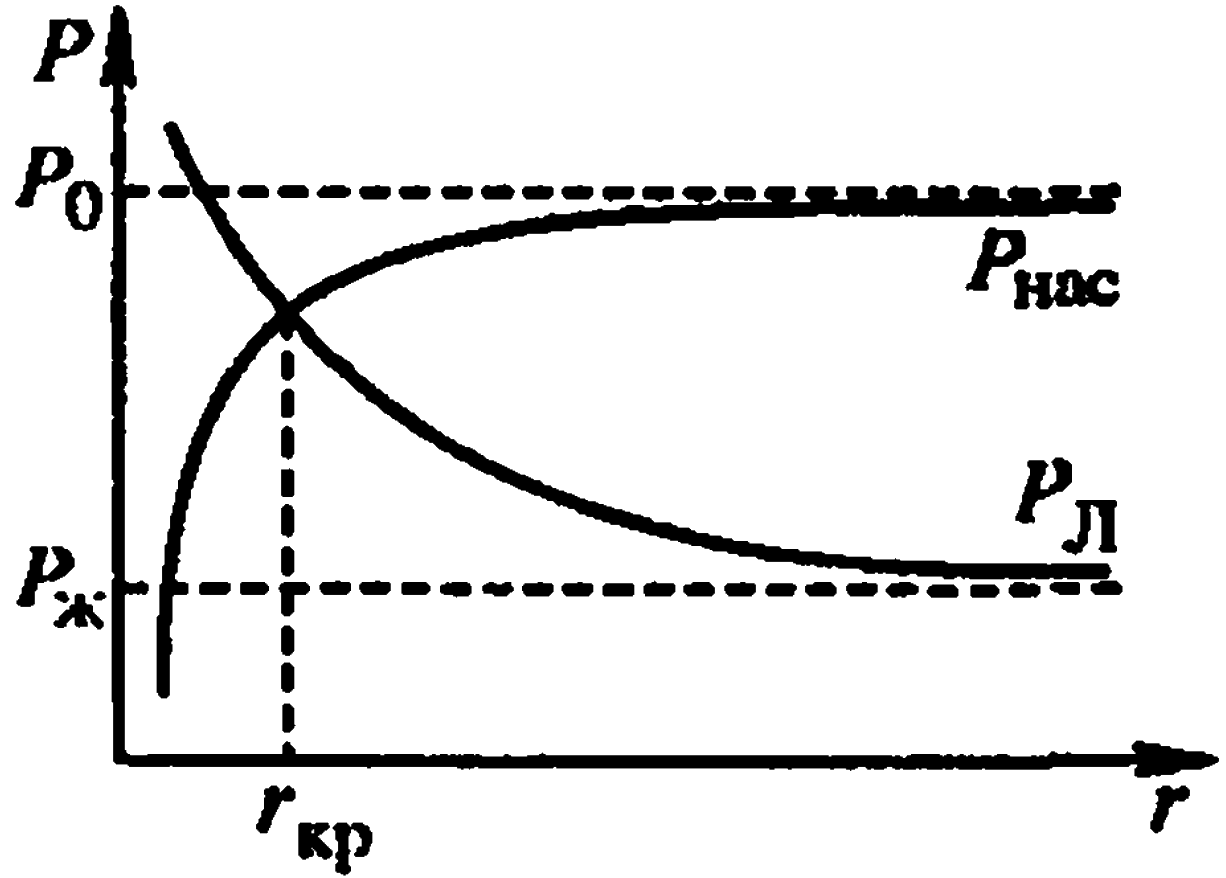
\includegraphics[width=42mm]{ris24.png}
\end{wrapfigure}
$$r_\text{кр.}\simeq\dfrac{2\sigma}{P_0(T)-P_\text{ж.}}\textbf{ --- критический размер пузырька}$$
При $r<r_\text{кр. }P_\text{нас.}<P_\text{лап.}\rightarrow$ пузырек не выдерживает и схлопывается.\\
При $r>r_\text{кр. }P_\text{нас.}>P_\text{лап.}\rightarrow$ пузырек начинает расти.\\[0.5cm]
Аналогичный случай --- капля воды в переохлажденном паре
$$r_\text{кр.}\simeq\dfrac{2\sigma}{P_0(T)-P_\text{п.}}\dfrac{v_\text{ж.}}{v_\text{п.}}$$
$r<r_\text{кр.}$ --- капля испарится, $r\geqslant r_\text{кр}$ --- будет расти.
\paragraph{Роль	зародышей в образовании новой фазы.} Если в очищенную от посторонних примесей воду, которая остается жидкой при $t=-10^\circ C$ и ниже бросить кристаллик льда (\textbf{зародыш} кристаллической фазы) или встряхнуть сосуд, то вода быстро затвердеет и ее температура быстро поднимется до $0^\circ C$. Если же она не была очищена от посторонних вкраплений, способных выполнять функцию зародыша кристаллической фазы, то переохлаждение наблюдаться не будет. (Подробнее --- Сивухин стр. 465-466).

       
 

\section{\normalsize Распределения Максвелла по проекциям и модулю скорости частиц. Наиболее вероятная, средняя и среднеквадратичная скорости.}
\paragraph{Распределения Максвелла по проекциям и модулю скорости частиц.} Газ состоит из большого числа $N$ тождественных молекул, находящихся в состоянии беспорядочного теплового движения при $T$. $\varphi(v_x)dv_x$ --- вероятность попадания проекции скорости молекулы в интервал $(v_x; v_x+dv_x)$. Найдем $f(v)=\varphi(v_x)\varphi(v_y)\varphi(v_z)$, предполагая, что попадание одной проекции в нужный интервал не зависит от других.\\
$\varphi(v)\sim e^{-\beta E}$, где $\beta=\frac{1}{KT}$, а так как молекулы обладают лишь кинетической энергией в нашей модели, то энергия одной частицы $E=\dfrac{mv^2}{2}$; $\int_{-\infty}^{+\infty}\varphi(v_x)dv_x=1$ --- условие нормировки.\\
$\varphi(v_x)=A\exp\left\{\frac{-mv_x^2}{2kT}\right\}\Rightarrow A\int_{-\infty}^{+\infty}\exp\left\{\frac{-mv_x^2}{2kT}\right\}dv_x=1\Leftrightarrow A=\left(\int_{-\infty}^{+\infty}\exp\left\{\frac{-mv_x^2}{2kT}\right\}dv_x\right)^{-1}$\\
\begin{multline*}
I=\int_{-\infty}^{\infty}e^{-x^2}dx\Rightarrow I^2=\int_{-\infty}^{+\infty}e^{-x^2}dx\infint e^{-y^2}dy=\infint\infint e^{-x^2+y^2}dxdy(dxdy=d\text{П})=\\=\int_{0}^{+\infty}e^{-r^2}2\pi rdr=2\pi\int_{0}^{+\infty}e^{-r^2}rdr=\left|\blacktriangleright z=r^2,\ dz=2rdr\blacktriangleleft\right|=\pi\int_{0}^{\infty}e^{-z}dz=-\pi e^{-z}|_0^\infty=\pi\Rightarrow\\\Rightarrow A^{-1}=\infint e^{-\frac{mv_x^2}{wkT}}dv_x=\left|\blacktriangleright z^2=\frac{mv_x^2}{2kT},\ dz=\sqrt{\frac{m}{2kT}}dv_x\blacktriangleleft\right|=\sqrt{\frac{2kT}{m}}\infint e^{-z^2}dz=\sqrt{\frac{2\pi kT}{m}}\Rightarrow\\\Rightarrow \varphi(v_x)=\sqrt{\frac{m}{2\pi kT}}e^\frac{-mv_x^2}{2kT}
\end{multline*}
$\varphi(v_x)=\sqrt{\frac{m}{2\pi kT}}e^\frac{-mv_x^2}{2kT}$\textbf{ --- закон распределения Максвелла по проекциям скоростей частиц.}\\
$F(v)=f(v_x)f(v_y)f(v_z)\cdot4\pi v^2=(\frac{m}{2\pi kT})^{3/2}\cdot4\pi v^2e^{-\frac{mv^2}{2kT}}$ --- \textbf{закон распределения Максвелла по абсолютным значениям скоростей.}\\
\paragraph{Наиболее вероятная, средняя и среднеквадратичная скорости.} 
\begin{enumerate}
	\item Наиболее вероятная скорость. $(F(v))'=0\Leftrightarrow2ve^{-\frac{mv^2}{2kT}}-2v^2\frac{mv}{2kT}e^{-\frac{mv^2}{2kT}}=0\Leftrightarrow v_\text{нв}=\frac{2kT}{m}$
	\item Средняя скорость.
	 $<v>=\int_{0}^{\infty}vF(v)dv=4\pi\sqrt{\frac{m}{2\pi kT}}^3\int_{0}^{\infty}e^{-\frac{mv^2}{2kT}}v^3dv$
	 \[I(\lambda)=\int_{0}^{\infty}e^{-\lambda z^2}zdz=\left|\blacktriangleright \lambda z^2=x,\ 2\lambda zdz=dx \blacktriangleleft\right|=\dfrac{1}{2\lambda}\int_{0}^{\infty}e^{-x}dx=\left.\frac{1}{2\lambda}(-e^x)\right|_0^\infty=\frac{1}{2\lambda} \Rightarrow\]
	 \[<v>=\int_{0}^{\infty}vF(v)dv=4\pi\left(\frac{m}{2\pi kT}\right)^{3/2}\frac{1}{2}\left(\frac{2kT}{m}\right)^2=\sqrt{\frac{8kT}{\pi m}} \]
	 \item Среднеквадратичная скорость. $\left< v^2 \right>=\int_{0}^{\infty}v^2F(v)dv=4\pi\left(\frac{m}{2\pi kT}\right)^{3/2}\int_{0}^{\infty}e^{-\frac{mv^2}{2kT}v^4dv}$
	 \[ I(\lambda)=\int_{0}^{\infty}e^{-\lambda z^2}dz=\left|\blacktriangleright x^2=\lambda z^2;\ dx=\sqrt{\lambda}dz \blacktriangleleft\right|=\frac{1}{\sqrt{\lambda}}\int_{0}^{\infty}e^{-x^2}dx=0.5\sqrt{\frac{\pi}{\lambda}}\]
	 \[\frac{d^2 I}{d\lambda^2}=\int_{0}^{\infty}e^{-\lambda z^2}z^4dz=\frac{3\pi}{8\lambda^{3/2}}\Rightarrow \left< v^2 \right>=4\pi\left(\frac{m}{2\pi kT}\right)^{3/2}\frac{3}{4}\frac{\sqrt{\pi}}{2}\left(\frac{2kT}{m}\right)^{5/2} =\frac{3kT}{m}\Rightarrow\] \[\Rightarrow v_\text{ср.кв.}\sqrt{\left< v^2\right>}=\sqrt{\frac{3kT}{m}} \]
	\end{enumerate}
        
 \section{\normalsize Распределение Максвелла по энергиям частиц. Средняя и наиболее вероятная энергии частиц.} 
\paragraph{Распределение Максвелла по энергиям частиц.} $E=\frac{mv^2}{2}\Leftrightarrow E=\sqrt{\frac{2E}{m}}\Rightarrow \\ \Rightarrow F(E)=\frac{2}{\sqrt{\pi *kT)^3}}\exp\left\{-\frac{E}{kT}\right\}\sqrt{E}.$
\paragraph{Средняя и наиболее вероятная энергия частиц.} 
\begin{enumerate}
	\item Наиболее вероятная энергия.
	\[(F(E))'=0\Leftrightarrow\frac{1}{2\sqrt{E}}e^{-\frac{E}{kT}}-\frac{1}{kT}e^{-\frac{E}{kT}}\sqrt{E}=0\Leftrightarrow E_\text{н.в.}=\frac{kT}{2}  \]
	\item Средняя энергия. 
	\[ \left<E\right>=\int_{0}^{\infty}EF(E)dE=\frac{2}{\sqrt{\pi (kT)^3}}\int_{0}^{\infty}e^{-\frac{E}{kT}}E^{3/2}dE= \frac{4}{\sqrt{\pi(kT)^3}}\int_{0}^{\infty}e^{-\frac{x^2}{kT}}x^4dx=\frac{3}{2}kT  \]
\end{enumerate} 
 
 \section{\normalsize  Среднее число молекул, сталкивающихся в единицу времени с единичной площадкой. Средняя энергия молекул, вылетающих в вакуум через малое отверстие.}
\paragraph{ Среднее число молекул, сталкивающихся в единицу времени с единичной площадкой.} 


\begin{wrapfigure}{L}{5cm}
	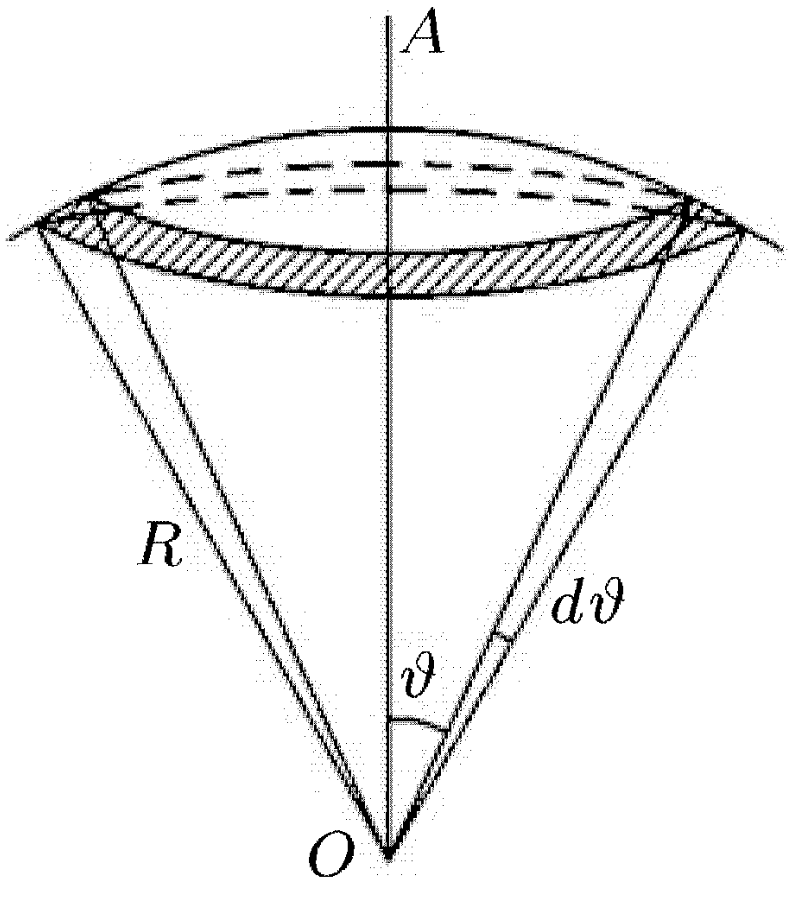
\includegraphics[width=50mm]{ris27.png}
\end{wrapfigure}$\;$\\
$\Omega = 2\pi(1-\cos\vartheta);\ d\Omega=2\pi\sin\vartheta\, d\vartheta;\\ dN=N\frac{d\Omega}{4\pi}=\frac{N}{2}\sin\vartheta\, d\vartheta$ --- среднее число молекул, направления скоростей которых лежат в пределах телесного угла $\Omega$ и образующие углы между $\vartheta$ и $\vartheta+d\vartheta$ с направление OA.\\
Выделим группу молекул с x-компонентами скоростей от $v_x$ до $v_x+dv_x$, $v_x>0$. Пусть их число в единице объема $dn_\vartheta$, тогда число их ударов о 1см$^2$ за 1с: $d\nu_\vartheta=dn_\vartheta v_x=\\=0.5n \sin \vartheta\cos\vartheta\,d\vartheta\,v$
\[d\nu_{\vartheta, v} =\frac{n}{2}\sin\vartheta\cos\vartheta d\vartheta v F(v)dv=\]\[=\frac{n}{2}\sin\vartheta\cos\vartheta d\vartheta v 4\pi v^2\left(\frac{m}{2\pi kT}\right)^{3/2}\exp\left(-\frac{mv^2}{2kT}\right)=\]\[=2\pi n\left(\frac{m}{2\pi kT}\right)^{3/2}\left[v^3 \exp\left(-\frac{mv^2}{2\pi kT}\right)dv\right]\left[sin \vartheta\cos\vartheta d\vartheta\right]\Rightarrow\]\[\Rightarrow \nu=2\pi n\left(\frac{m}{2\pi kT}\right)^{3/2}\int_{0}^{\infty}v^3\exp\left(-\frac{mv^2}{2kT}\right)dv\int_{0}^{\pi/2}\sin\vartheta\cos\vartheta d\vartheta=\frac{n\overline{v}}{4}   \]
\paragraph{ Средняя энергия молекул, вылетающих в вакуум через малое отверстие.} Будем рассматривать одноатомный газ. $dn$ --- число молекул в 1 см$^3$, обладающих скоростью в интервале $(v,v+dv)\Rightarrow dn=nF(v)dv$.\\
За 1 секунду из отверстия вылетает $1/4dn\,v$, которые унесут $\frac{mv^2}{2}1/4dn\,v\Rightarrow$
\[ \Rightarrow E_\text{полн.}=\int1/4\frac{mv^2}{2}dn\,v=\int_{0}^{\infty}\frac{m}{8}v^3nF(v)dv\Rightarrow \overline{E_\text{выл.}}=\frac{E_\text{полн.}}{\int_{0}^{\infty}1/4nvF(V)dv}=\]\[=\frac{m/2\int_{0}^{\infty}v^5e^{-\lambda v^2}dv}{\int_{0}^{\infty}v^3e^{-\lambda v^2dv}}=\frac{m}{\lambda}=2kT   \]
  
 \section{\normalsize Распределение Больцмана. Барометрическая формула.} Пусть $\mathbf{f}$ --- объемная сила в расчете на одну частицу. Выделим в газе элемент объема толщиной $dz$ и площадью основания $S$. В этом элементе находится $dN=nSdz$ частиц, где $n$ --- объемная плотность числа частиц. Условие механического равновесия слоя имеет вид:
\[f_zdN+P(z)dS-P(z+dz)S=0\text{ или }\frac{\partial P}{\partial z}=f_zn  \] 
Пусть сила $\mathbf{f}$ --- потенциальная, $\mathbf{f}$ $=-\text{grad}\,u(\mathbf{r})$, $f_z=-\frac{\partial u}{\partial z}$. Тогда для идеального газа при $T=const$ отсюда следует
\[\frac{\partial P}{\partial z}=-\frac{\partial u}{\partial z}\frac{P}{kT}\Rightarrow\frac{\partial(\ln P)}{\partial z}=-\frac{\partial}{\partial z}\left(\frac{u}{kT}\right)\Rightarrow P=P_0\exp\left(-\frac{u}{kT}\right) \]
Для частного случая однородного поля тяжести $\mathbf{f}=m\mathbf{g}$ потенциальная энергия равна $u=-m\mathbf{gr}=mgz$. Тогда
\[P=P_0\exp\left(-\frac{mgz}{kT}\right).  \]
Это соотношение называется \textbf{барометрической формулой}.\\
Поскольку $P=nkT$, то распределение плотности числа частиц $n$ идеального газа в потенциальном поле имеет вид
\begin{equation}
\label{eq:bolz1}
n=n_0\exp\left(-\frac{u}{kT}\right)
\end{equation}
Это распределение дает средние значения плотности, поскольку состояние равновесия динамическое и возможны отклонения от среднего (флуктуации) в какие-то моменты времени.\\
Для числа частиц $dN=ndV$, находящихся в элементе объема $dV$, из \eqref{eq:bolz1} следует
\begin{equation}
\label{eq:bolz2}
dN=n_0\exp\left(-\frac{u}{kT}\right)dV.
\end{equation}
Соотношения \eqref{eq:bolz1} и \eqref{eq:bolz2} называются \textbf{распределением Больцмана.}
   
 \section{\normalsize Микро- и макросостояния. Статистический вес. Распределение Гиббса.}
\paragraph{Микро- и макросостояния.} \textbf{Микроскопическое состояние} --- состояние системы, определяемое заданием координат и импульсов.\\
\textbf{Макроскопическое состояние} --- состояние системы, характеризующееся небольшим числом макропараметров($P$, $V$, $T$, $\rho$, $\eta$ и т.д.).\\
Одно макросостояние может быть реализовано большим числом микросостояний за счете перестановки частиц, не меняющей наблюдаемого состояния.
\paragraph{Статистический вес.} Если система состоит из $N$ частиц, тогда $6N$ чисел полностью характеризует её состояние ($3N$ координат и $3N$ импульсов). Разобьем 6-ти мерный фазовый объем фазовый объем $V$ на $m$ ячеек $V_1,\ldots,V_m$. Каждая молекула находится в какой-то ячейке $N_1,\ldots,N_m$\\
$P_i=\frac{V_i}{V}$ --- вероятность попасть в $i$-ую ячейку для каждой частицы, если в $i$-ой ячейке $N_i$ молекул, то $P_i=\left(\frac{V_i}{V}\right)^{N_i}.$ Все микросостояния $P_1^{N_1}\times\ldots\times P_m^{N_m}$, а если $V_i=v,~\forall~i=~\overline{1,m}$, то $\left(\frac{v}{V}\right)^N$. Все частицы тождественны, значит число способов реализовать данное макросостояние: $G=\frac{N!}{N_1!\ldots N_m!}$ --- \textbf{Статистический вес}.\\
\textbf{Статистический вес} --- число равновероятностных микросостояний, каждое из которых реализует данное макросостояние, то есть термодинамическая вероятность данного распределения $P=GP_1^{N_1}\times\ldots\times P_m^{N_m}$, а в случае одинаковых ячеек $\left(\frac{v}{V}\right)^N=const\Rightarrow P=G$ (с точностью до константы).
\paragraph{Распределение Гиббса.} Он пока не зашел, если что 80-82 страницы Кириченко. Завтра перенесу.
 
 \section{\normalsize Статистическое определение энтропии. Аддитивность энтропии. Закон возрастания энтропии.} 
\paragraph{Статистическое определение энтропии.} $S=k_\text{Б.}\ln G$.
\paragraph{Аддитивность энтропии.} Разобьем систему на 2 подсистемы со статистическими весами $G_1$ и $G_2$. Если взаимодействие между ними слабое, то микросостояния у них меняются независимо, тогда $G=G_1\cdot G_2$	--- статистический вес системы. Тогда $S=k\ln G_1+ k\ln G_2=S_1+S_2$ --- свойство аддитивности. В общем случае: $S=k\ln G=k \ln N!-\sum_{i=1}^{m}k\ln N_i!=\\=\left|\blacktriangleright\ln N!\simeq N\ln N-N\blacktriangleleft\right|=kN\ln N-\cancel{kN}-k\sum_{i=1}^{m}N_i\ln N_i+\cancel{k\sum_{i=1}^{m}N_i}=kN\left(\ln N-\sum_{i=1}^{m}\frac{N_i}{N}\ln N_i\right)=\\=kN\left(\cancel{\ln N}-\sum_{i=1}^{m}W_i\ln W_i-\cancel{\ln N\sum_{i=1}^{m}W_i}\right)=-kN \sum_{i=1}^{m}W_i\ln W_i$
\[
S=-kN\sum_{i=1}^{m}W_i\ln W_i
\]
\paragraph{Закон возрастания энтропии.} Среди всех направлений эволюции системы предположительным является то, при котором вероятность состояния оказывается наибольшей, тогда
\begin{enumerate}
	\item с наибольшей вероятностью энтропия замкнутой системы не убывает: $\frac{dS}{dt}\geqslant0$;
	\item в состоянии термодинамического равновесия (наиболее вероятное) энтропия максимальна $S=S_{max}; \frac{dS}{dT}=0$
\end{enumerate}
Хотя, если энтропия в какой-то момент достигла своего максимума, то почти наверняка в следующий момент времени она уменьшится. Таким образом энтропия системы, находящейся с макро- точки зрения в состоянии термодинамического равновесия, совершает небольшие колебания.
  
 \section{\normalsize Изменение энтропии при смешении газов. Парадокс Гиббса.}
\paragraph{Изменение энтропии при смешении газов.} Пусть два идеальных газа 1 и 2 заключены в закрытом сосуде с твердыми адиабатическими стенками, так что $V=const$. Также пусть они разделены перегородкой, состоящей из двух: $a$ пропускает 1, но не пропускает 2, а $b$ --- наоборот. Температуру в сосуде поддерживаем постоянной и равной $T$. Удалим перегородку $b$, тогда $\Delta S_1=\nu_1R\ln \frac{V}{V_1}$, при этом состояние газа 2 не изменится. Теперь удалим перегородку $a$, тогда $\Delta S_2=\nu_2R\ln \frac{V}{V_2}$, аналогично состояние газа 2 не изменится.

\begin{wrapfigure}{l}{30 mm}
	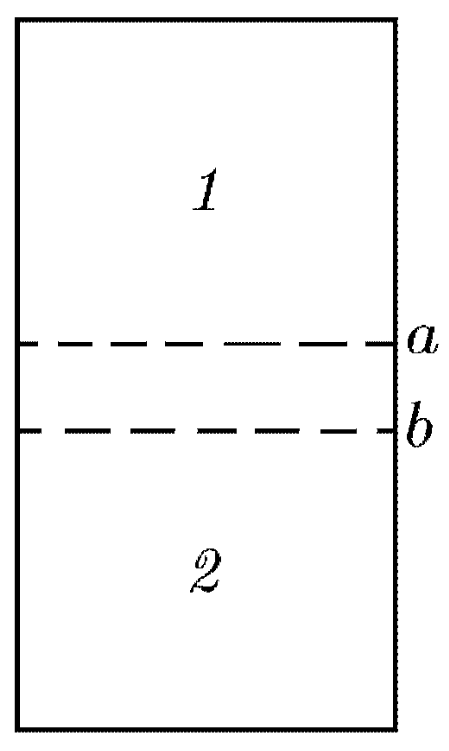
\includegraphics[width=30mm]{ris31.png}	
\end{wrapfigure}
 Таким образом мы квазистатически смешаем 2 газа и 
\begin{equation}
\label{eq:entrop}
 \Delta S=\Delta S_1 + \Delta S_2=R\left(\nu_1 \ln \frac{V}{V_1}+\nu_2\ln \frac{V}{V_2}\right)>0
 \end{equation}
 Но если же газы тождественны ($\nu_1=\nu_2=\nu/2;\ V_1=V_2=V/2$), то по формуле $\Delta S=\nu R \ln 2$, однако конечное состояние макроскопически ничем не отличается от начального. Энтропия возросла, а состояние системы не изменилось. В этом и есть \textbf{парадокс Гиббса.}\\
 \eqref{eq:entrop} выведена для случая смешивания существенно различных газов. Для тождественных газов рассуждения неприменимы. Принципиально невозможно квазистическок перемешивание тождественных газов вышеописанным способом.
\end{document}
